%COPYRIGHT!!!!!


\documentclass[12 pt, a4paper]{article}


\usepackage[style=numeric, backend=biber,sortcites,]{biblatex}
\bibliography{kilder.bib}

\usepackage[english]{babel}  								% For norsk oppsett
\usepackage[utf8]{inputenc}
\usepackage{amsmath}
\usepackage{amssymb}
\usepackage{graphicx}
\usepackage{chemformula}
\usepackage{tabularx}
\usepackage{subcaption}
\usepackage{hyperref}
\usepackage{fancyhdr}
\usepackage{enumerate}
\usepackage{float}
\usepackage{tikz}
\usepackage{fancyhdr}
\usepackage{lastpage}
\usepackage{comment}
\usepackage{circuitikz}
\usepackage{physics}
\usepackage[includeheadfoot, margin =0.5 in]{geometry}
\usepackage[FYS, OnlyFrontpage]{mnfrontpage} 			%SKIFT HER!!!
\usepackage[version=3]{mhchem}
%\usepackage{biblatex}%,style=numeric-comp
%\usepackage{cite}
\usepackage{siunitx}
\usepackage{todonotes}
\usepackage{xcolor}
\usepackage{listings}
%%%%
\usepackage[bottom]{footmisc}
\renewcommand\footnoterule{\rule{\linewidth}{0.5pt}}
%\renewcommand[\footnoterule]{%
%	\kern -3pt
%	\hrule width \textwidth height 1pt
%	\kern 2pt
%}
%%%%
\lstset{basicstyle=\ttfamily,
  showstringspaces=false,
  commentstyle=\color{red},
  keywordstyle=\color{blue}
}
%\usepackage{showframe}  %Dette viser hvordan strukturen på sidene er


\author{Sondre Torp  - Sondrt@student.matnat.uio.no }


%\addbibresource{kilder.bib}
%
%\documentclass[a4paper, 12pt, norsk]{article}
%\usepackage[english]{babel}
%\usepackage[utf8]{inputenc}
%\usepackage[T1]{fontenc}
%\usepackage{graphicx}
%\usepackage{siunitx}
%\usepackage[usenames,dvipsnames,svgnames,table]{xcolor}
%\usepackage{listings}
%\usepackage{float}
%\usepackage{fancyhdr}
%\usepackage[includeheadfoot, margin =1 in]{geometry}
%\usepackage[FYS, OnlyFrontpage]{mnfrontpage}
%\usepackage{hyperref}
%\usepackage{amsmath}
%\usepackage{multirow}
%\usepackage{caption}
%\usepackage{subcaption}
%\usepackage{enumitem}
%\usepackage{amsmath,amssymb}
%\usepackage{todonotes}
%\renewcommand{\exp}[1]{\mathrm{e}^{#1}}
%\renewcommand{\i}{\mathrm{i}}
%\usepackage{tikz}
%\usepackage{booktabs}
%\usepackage{babel, csquotes, newcent, textcomp}
%
%\bibliography{kilder.bib}
%%\usepackage{lastpage}
%%\usepackage{showframe}  %Dette viser hvordan strukturen på sidene er
%
%
%
%\author{Sondre Torp  - Sondrt@student.matnat.uio.no }
%

%\documentclass{book}
\usepackage{indentfirst}
\usepackage{hyperref}


\newcommand\myworries[1]{\textcolor{red}{#1}}

\usepackage{babel, csquotes, newcent, textcomp}
%\usepackage[backend=biber, sortcites]{biblatex}
%\addbibresource{kilder.bib}

\usepackage{titlesec}

\titleformat{\section}
  {\normalfont\fontsize{16}{19}\bfseries}{\thesection}{1em}{}
\titleformat{\subsection}
  {\normalfont\fontsize{14}{17}\bfseries}{\thesubsection}{1em}{}
\titleformat{\subsubsection}
  {\normalfont\fontsize{14}{17}\selectfont}{\thesubsubsection}{1em}{}


\numberwithin{equation}{section}






%-------------------------------------------------------------------- Doc starts here

\title{Sondres master utkast 16.01.2020 }
\pagenumbering{roman}	%Roman numbering of pages.
\begin{document}
	\mnfrontpage

\pagestyle{fancy}
\fancyhf{}
\rhead{Master!}
\lhead{Sondre Torp}
\fancyfoot[CE,CO]{\roman{page}}      %\number\value{page}}


\renewcommand{\headrulewidth}{2pt}
\renewcommand{\footrulewidth}{1pt}

\setlength{\parindent}{2em}
\setlength{\parskip}{1em}
\renewcommand{\baselinestretch}{1.5}


\setcounter{page}{1}
\pagebreak
\part*{Abstract}
%Abstract
%\thispagestyle{empty}

This is the Abstract!



\mbox{}
\vfill
© Copyright by Sondre Torp\\



\pagebreak

\part*{Acknowledgements}
%\thispagestyle{empty}

I like to acknowledge ... Sabrina!

UOC

Georges 

m.m.


\pagebreak


\tableofcontents
\listoffigures
\listoftables

\pagebreak

\pagenumbering{arabic}	%Numbering of pages

\fancyfoot[CE,LO]{\leftmark}
\fancyfoot[LE,RO]{Page \number\value{page} of \pageref{LastPage}}
\fancyfoot[CE,CO]{ }

\part{Introduction}
\section{Introduction and Overview}
%Introduce the task at hand.

	This work focus in Machine Learning (\ac{ML}) applied in the field of batteries. Specifically, a new method is developed to predict chemical properties like voltage, capacity and energy density of chosen electrode materials.

	In the introduction a general background for this work will be given. The chapter includes a motivation, the scope of the thesis and its structure. 
 

\subsection{Motivation}
%*) Why batteries are important (i.e. cell phones, cars). 

The motivation for this work originates from the rapidly increasing demand for improved batteries, both for vehicular and stationary applications, with longer life, lower cost, and adequate energy storage options.

%\myworries{elaborate more on predictive modeling ... }

%Clarify what you want to cover. 
%Write more about: PV, wind, solar -> storage.

%"At what cost can one charge stationary secondary batteries with solar/wind power efficiently, and provide a centralized energy storage? For what shelf and cycle life? with how rapid a respons  a power outage or fluctuation in the grid. And with how large a capacity, at a competitive cost? " \myworries{where?}


%Why batteries are important(Cars how many in how long? )
Batteries are vastly complex and much efforts have been devoted to their development, in recent times \cite{blomgren2016development} \cite{hosaka2020research} \cite{cao2020batteries}, and even 3-D printed batteries are on the rise \cite{pang2020additive}. Yet, with all the efforts put in to electrochemical cells, there are still a never ending chase for batteries that can push the limits of their properties even further. The demand for better batteries are growing faster then ever. The global electric car fleet, for instance, is exceeding 5.1 million , almost doubling the number of new electric car registrations in the last year. According to the EV30@30 Scenario \cite{international2018global} the aim is to reach a $30\%$ market share for electric vehicles (\ac{EV}) in all models except two wheelers by 2030. This is because more than one quarter of global greenhouse gas emissions comes from this sector alone. The EV sales per year are then predicted to be more then 43 milion, and the stock numbering more than 250 milion. It is clear that millions of EVs will push the demands on the battery technology sector \cite{xiong2020overview}, with the market requiring high capacity and energy density batteries. 


%*) What are the most important properties that todays batteries should improved (i.e. higher capacities, longer life times (durability) etc.)
Some of the most desirable cell properties are; voltage, energy density, specific energy or capacity, flammability, available cell constructions, operating temperature range, shelf life or self discharge, low cost, and worldwide consumer distribution. Most of these properties are to an extent dictated by battery chemistry. Due to the complexity of the chemical processes involved, it is of high importance to be able to develop predictive modeling methods to search for better compositions and performance. In this work we will develop a method to predict; voltage, energy density, specific energy, and the physical stability of materials as electrodes.


%*) What is a typical procedure for designing a new battery ( a general discussion from the experimental and theoretical point of view)
%The idea behind the design of a battery is fairly simple, due to their similar procedure to create electricity. Two of the most important parts are the Anode and the Cathode. A cell produces electricity when placed into a medium that has conductive properties, namely the electrolyte.


%*) Focus on the theoretical part. What theoretical techniques are used today for the design of new batteries (i.e. DFT calculations,  molecular dynamics simulations etc). Provide some references.

Today some of the main methods for theoretical advances in battery science are density functional theory (\ac{DFT}), molecular dynamic (\ac{MD}) simulations and machine learning. In the field of computational materials science, a large amount of both theoretical and experimental data has been generated during the last couple of decades. This is due to the success of DFT, MD simulations and the increase in computational power. These methods combined with the high-throughput (\ac{HT}) approach have generated a lot of data and made it, in cooperation with big projects like the Materials Genome Initiative, easily available. DFT is a cornerstone for simulation procedure in material science \cite{schleder2019dft} \cite{pour2011structural} \cite{kirklin2013high}, while MD simulation is, among other things, know to be well suited to explore solid-state materials at the atomic level \cite{kaneko2003local} \cite{ammundsen1999lattice} \cite{islam2000atomistic} \cite{braithwaite2000computational}. 

%*) Make clear if the theoretical results provide useful information during the whole process of building a new battery.


%*) Start discussing that experimental and traditional theoretical approaches are expensive and computationally demanding. From that point on start introducing the need of new theoretical approaches

The experimental and traditional approaches to improving battery technology come with a high cost and time-consuming procedures of synthesis. Different applications are usually locked to one type of material because of the investment associated with large-scale production. Changing material is thus rare, and viewed as a revolution. This is why the success of the initial material selected in one sector is crucial for that technology's lasting success. Many new inventions, with close following niches of technologies, demand the development of their own material set with properties tailored to that specific technology. Properties from compatibility to toxicity are essential and make the search for materials into a multi-dimensional problem \cite{curtarolo2013high}. 

Traditional computational methods, like DFT and MD, come with a high computational cost compared with machine learning methods. ML uses past data to find relations and correlations in between the data. Based on them, the models (ML models) created can be used for prediction in new unknown materials. For a ML model to be accurate there are two requirements; a large set of data, often referred to as "big data", and that the model is given the right descriptors. Big data, in the form of material databases already exist, like Material Project (\ac{MP}) \cite{Jain2013}, AFLOWLIB consortium \cite{curtarolo2012aflowlib}, OQMD \cite{saal2013materials}, NOMAD \cite{draxl2018nomad}, and others \cite{schleder2019dft}.  

The advantages of the ML approach are several - it is computational efficient - it only takes a few minutes/hours to build a model, and seconds to making predictions. One example of a ML approach towards  the search of novel materials are exemplified in Sendek et al., where their ML approach took $<1$ second per prediction, while their DFT approach took approximately four weeks per prediction, on solid Li-ion conducting materials \cite{sendek2018machine}. 

Another advantage of a ML approach is that no mathematical or physical relation, and no laws of nature is needed for a good predictions. The ML model will find these relations, but for most of the models these relations are difficult to interpret. In principle a ML algorithm can be given any information (input), and if some of the information is irrelevant, then the ML algorithm will give zero weight to that information. However, if only a part of the relevant information is given to the ML algorithm, the model will not give good predictions.  

There are a couple of challenges of using ML models, as mentioned, a need for big data and a sufficient amount of \textit{examples}. The accuracy of the said data is important, since without accurate data there are no accurate predictions. Descriptors need to be formulated in such a way that the ML model understands the input. Lastly, the choice of classifier is of importance, i.e. Random forest, Support Vector Regression (\ac{SVR}), neural networks, etc.  

In real physical or chemical problems, the ML method can provide good estimations, but these are not exact predictions. There are several reason for this, i.e. small training examples, accuracy of the training data, not providing all relevant descriptors etc.  However, a good ML model can provide us with the most promising materials for a given application, or as a minimum, significantly reduce the number of material candidates that experimental studies should focus on. 

\subsection{Scope of the thesis}
This work aims to develop a methodology to predict selected battery properties accurately without the need of large scale simulations, or computer heavy calculations. Using state-of-the-art machine learning, and base properties taken from the existing database Materials Project, we propose a set of predictors to discover the properties of new, not yet explored electrodes, or even new properties in already well known electrodes. The properties used as targets for our predictions are; average voltage, gravimetric and volumetric capacity, specific energy, energy density and the stability of the materials. More specifically, this work look at the theoretical values of the given targets, and not experimental values. 
	
	The main objective of this thesis is to acquire knowledge about which features should be included for electrode predictions of the given targets by investigating a range of possible inputs, their configurations and their effect on prediction accuracy. It examines both features found in the Material Project database, and uncommonly used features in literature. In our opinion, a general examination of possible features for electrodes are lacking in research. Knowledge of which features improve prediction accuracy is useful in several ways. Even though material data generation is done faster then ever before, data acquisition and formatting can be time consuming, especially if an abundance of data is used. It can therefore be of great value to know what type of data that should be prioritized, and give focus to the areas we know will improve our predictions. This saves time from gathering data and testing. Knowledge about properties required can also expose, both, the effectiveness of less obvious features, that can be overlooked by other developers of ML-models, and the need for not yet introduced characteristics. Reducing the number of features will also reduce the complexity of the model, which saves energy and time. This work tries out different sets of features which should be considered when doing predictions on electrode materials.

%*) Start describing what are the goals of the present work. Give first the battery properties that you consider more important (e.g. capacity). The goal of the work is more or less the following (expand it): can the use as ML descriptors (input) of elemental atomic properties (e.g. atomization energy), and compounds properties (e.g. geometrical features, AP_RDF) can provide reasonable predictions for your goals. 


\subsubsection{Research Question} \label{sec:RQ}

Specifically, this work seeks to answer the following questions: 

\textbf{\ac{RQ}1:} Is there potential for the of use machine learning to improve the search for good battery materials?

\textbf{RQ2:} What predictors are suited for such a task?

\textbf{RQ3:} Does features overlap? What features should be removed from the feature space to achieve the most efficient training?

\textbf{RQ4:} How does the size of the database affect the results?

\textbf{RQ5:} Which ML method would be the most optimal for such a search?

%\textbf{RQ6:} Does the features proposed function for other materials or are they limited to electrode materials 

\subsubsection{Approach}

RQ1 regards the need to establish a database that is comprehensive enough to be of value for the selected machine learning method, and it must have the relevant information needed to get good predictions.

RQ2 concerns the choice of features examined in this work. They are inspired by a survey done on a similar project especially in the field of Metal Organic Framework (\ac{MOFS}) preformed by collaborators from the university of Crete \cite{fanourgakis2019robust} \cite{fanourgakis2020universal} and another research project done on MOFS by Fernandez et al.\cite{fernandez2013atomic}. Our choice of predictors were also, to a degree, dictated by the lack of more data, the difficulty of finding said data, and by the data we had. 

Regarding what descriptors applied, first we used physical descriptors, such as geometrical properties(volume, number of sites, etc.) of the unit cell. This because it was greatly efficient in similar studies on MOFS, and it is straightforward. Other descriptors were needed, and the void fraction seemed like a good candidate due to the nature of intercalation type batteries, and that both a geometrical feature and computationally cheap to obtain. We still needed a more chemical approach without doing large DFT type calculations, so we tried to make an atomic property weighted radial distribution function - approach, to include listed values like electronegativity, van der waals volume and magnetization. Before lastly, using the already known results, or targets, to make predictions on the other targets. That are more easily obtainable, with DFT, to account for the missing chemical intuition.

RQ3 examines the evaluation of the features space and how to limit its size. To achieve the most effective training principal component analysis was applied, thus systematically removing the redundancy within features. This is statistical procedure that uses a orthogonal transformation on the data to make a set of linearly uncorrelated variables and rank these after variance. 

RQ4 concerns the size of the database. All of the features were tested alone, and up against each other, both for a smaller database of Mg-ion intercalation batteries, and a bigger database of Li-ion intercalation batteries. The results of these two different databases might not be purely comparable, but due to the algorithm mainly using fundamental properties we will compare the results and look for trends as our database increases in size. 

RQ5 is approached as follows: Which machine learning method is more likely to yield correlation in our data?

\subsection{Structure of the thesis}
In this section a short presentation of how this thesis is structured is given. 

\noindent{\textbf{Part II: Foundation}}

\noindent{\textbf{Chapter 2: Batteries}}

	In this chapter a short history of batteries and their evolution are given, before going deeper into the state-of-the-art of Li ion batteries. An introduction to the theory of battery cells, their operation principles and design, is given. Before the battery properties of particular interest and their features related to this work, are presented. 

\noindent{\textbf{Chapter 3: Machine Learning}}

This chapter introduces the field of machine learning along with some key concepts. Challenges concerning the application of machine learning are also discussed. The subgroup of machine learning algorithms ensemble methods are introduced in the context of decision trees with a special emphasis on Random forest.The evaluation methods used in this work (e.g. root mean square error deviation, K-fold cross validation, etc.), as well as principle component analysis are presented. And Finally a introduction to state-of-the-art computational material design with an emphasis on electrodes and battery related works, are given. 


\noindent{\textbf{Part III: Experimental method}}

\noindent{\textbf{Chapter 4: Method}}

This works relies on data from the materials project database. These datasets are introduced in this chapter, as well as the features we used for our analysis, and a brief touch on the preprocessing of the data. Lastly the experimental environment is explained with the prediction pipeline. 


\noindent{\textbf{Part IV: Results and discussion }}

\noindent{\textbf{Chapter 5: Results}}

This chapter presents and discuss results for RQ1, RQ2, RQ3 and RQ4 with experiments performed for both databases and predictors on all targets. The first section of the chapter investigates the predictors one by one, and compare their results on the different databases. All the calculations are available on github (\url{https://github.com/sondrt/Creten_Stuff} \cite{github}).


\noindent{\textbf{Part V: Summary}}

\noindent{\textbf{Chapter 6: Conclusion and future work}}

In this chapter the most important finding from this research are revisited and put into perspective. In addition, suggestions for future work are laid out.




\pagebreak
\part{Foundations}
\section{Batteries}
 	This section presents a brief summary of some of the major steps in the history and evolution of batteries, with a description of lithium and magnesium-ion batteries and their role in todays market. The basic principles of batteries will be explained, with a special emphasis on electrodes. Lastly, some of the chemical properties related to this work will be introduced. 

\subsection{History and evolution of batteries}
One of the main issues regarding the development of sustainable and clean-energy technologies are the lack of efficient energy systems \cite{curtarolo2013high}. A tremendous amount of resources are used on an international level to produce batteries with higher capacity, voltage and energy density. The evolution of batteries started in Italy with Alessandro Volta (1745 - 1827). He built the first known battery in the year 1800 \cite{volta1800electricity}. His invention consisted of the voltaic pile, with zinc and copper plates stacked on top of each other and sheets of  brine-soaked cardboard between each plate. The revolutionary property of the voltaic pile was that it could produce a stable current for longer periods of time, not just short sparks of electricity. This invention was the foundation of todays modern battery (figure \ref{fig:voltaicpile}).

\begin{figure}[ht]
    \centering
    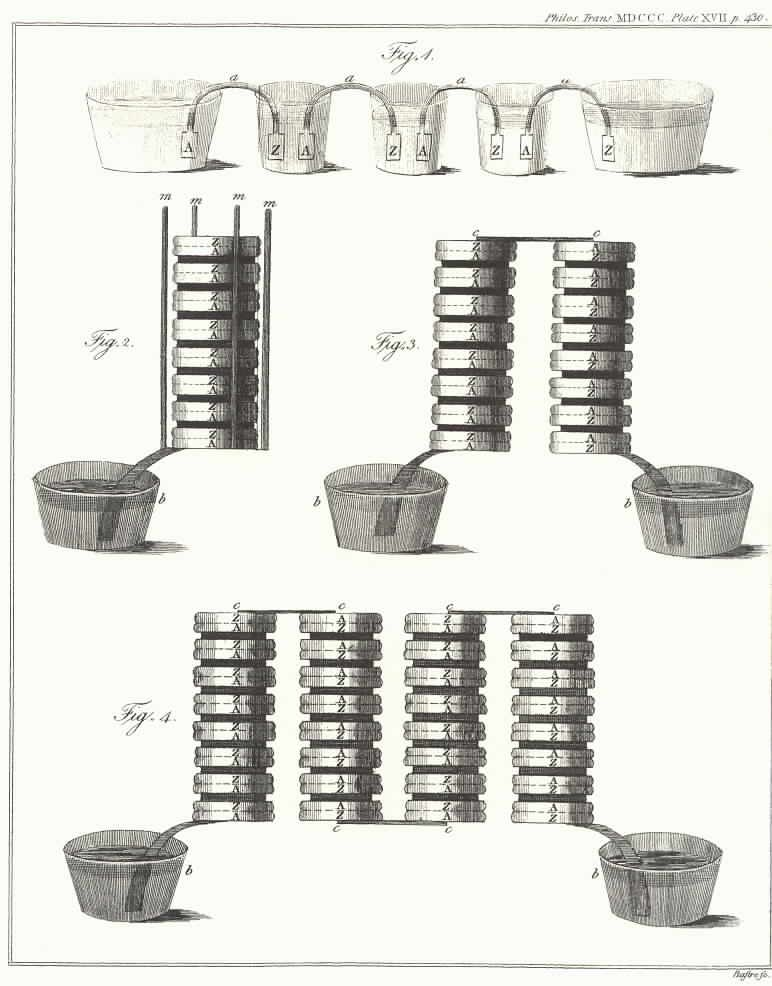
\includegraphics[width=0.5\textwidth]{volta.jpg}
    \caption{A voltaic pile, the first battery \cite{decker2005volta}}
    \label{fig:voltaicpile}
\end{figure}

Almost $40$ years later the British inventor John Frederic Daniell Volta continued this line of work, with the discovery of the Daniell cell \cite{daniell1836xi} in 1836. The Daniell cell, as illustraited in figure \ref{fig:DaniellCell}), is constructed with two half cells, one with a zinc electrode in a zinc sulfate dissolution, and a copper electrode in a copper sulfate solution. These half cells are connected by a salt bridge. The cell could give a voltage of $\SI{1.1}{V}$ through the reaction shown below \ref{eq:Daniell}. 


\begin{align}\label{eq:Daniell}
\ce{Zn_{(s)}} + \ce{Cu^{2+}_{(aq)}} \rightarrow \ce{Zn^2+_{(aq)}} + \ce{Cu_{(s)}} 
\end{align}

\begin{figure}[ht]
    \centering
    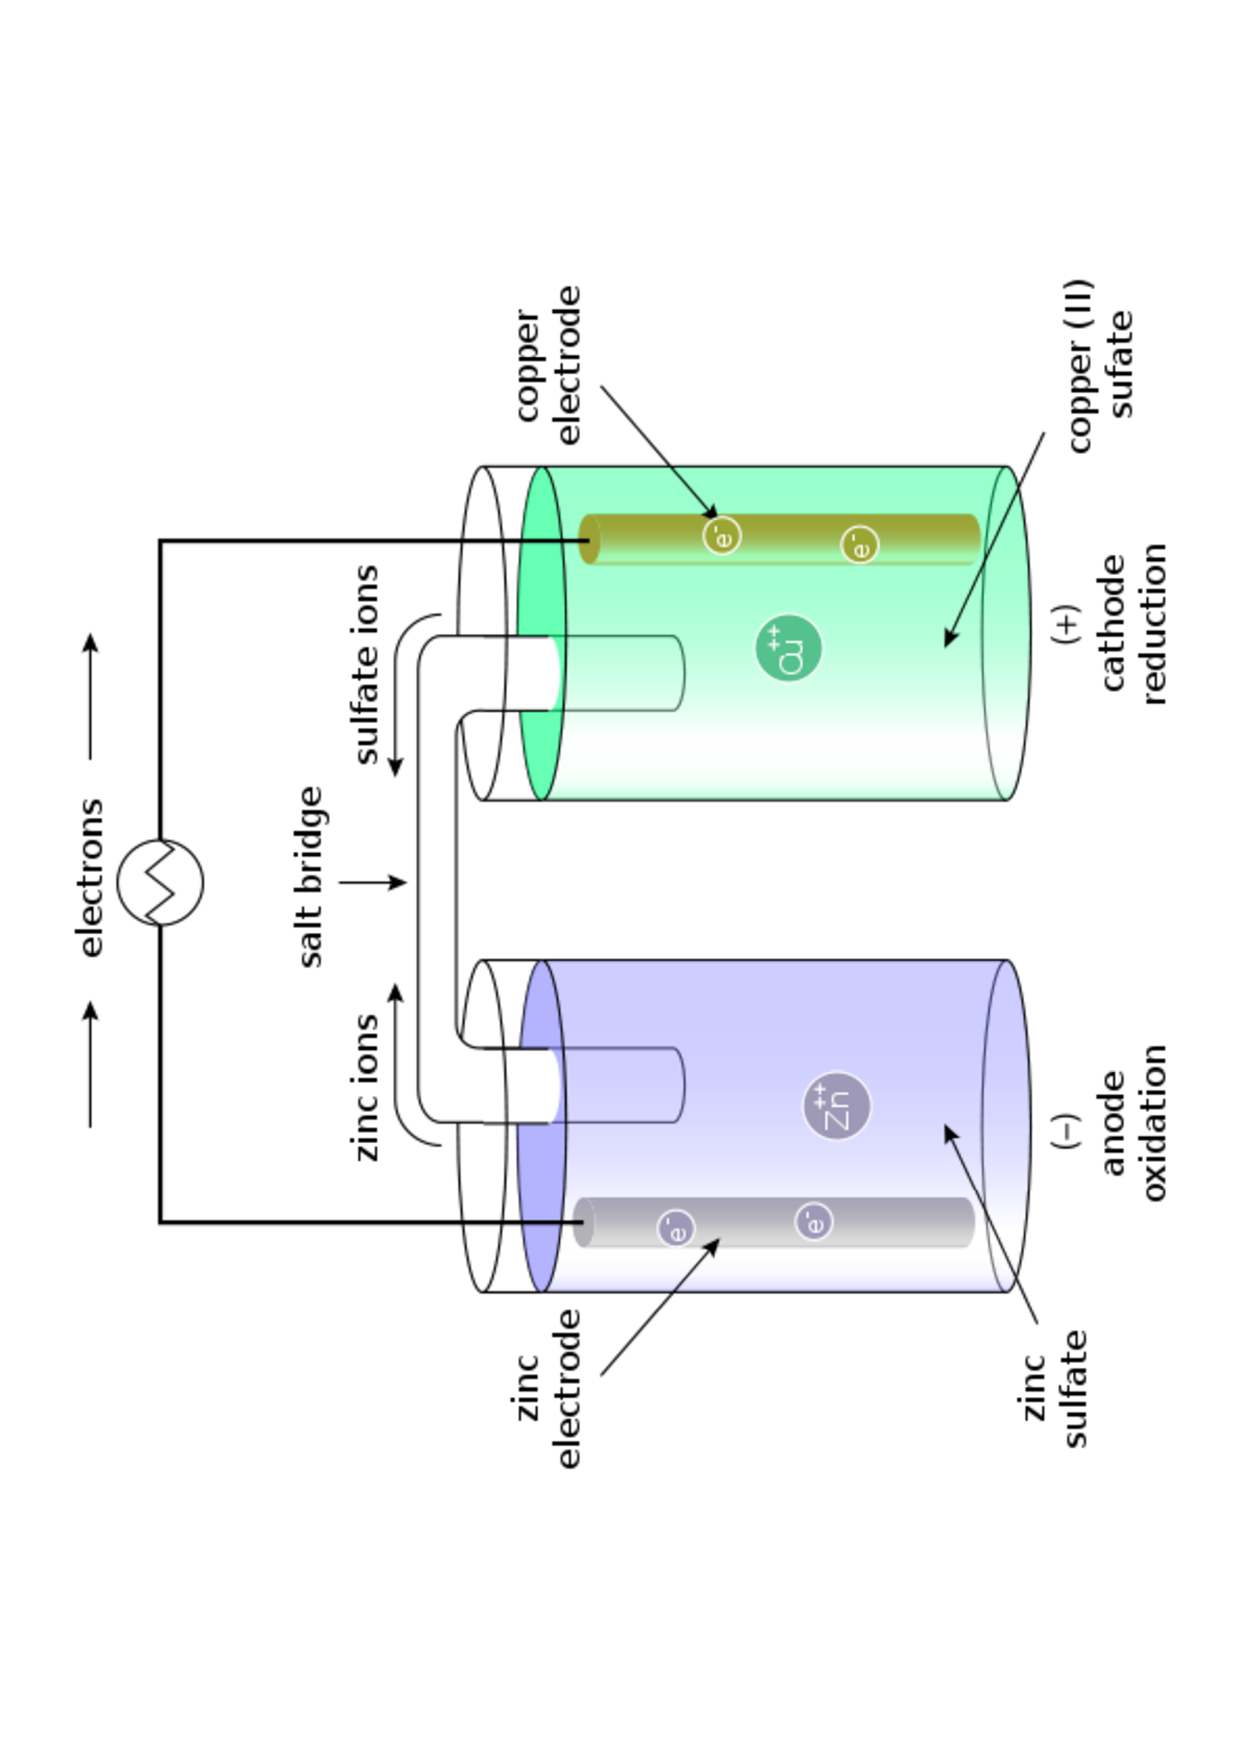
\includegraphics[angle=270,width=0.8\textwidth]{600px-Galvanic_cell_labeled.pdf}
    \caption[format=plain]{A draft of a Daniell cell. The anode is a piece of zinc and the cathode a piece of copper. The salt bridge transports ions between the solutions and the electrons moves through an external circuit \cite{wiki:Daniellcell}. }
    \label{fig:DaniellCell}
\end{figure}


In 1859 the French physicist Gaston Planté built the first led-acid battery. The battery could be charged by applying an external opposite potential, and it was the first secondary battery every made. Planté rolled two led plates into a spiral, separated by rubber strips, so that the plates would not touch. The lead-acid battery was special due to the electrolyte being an active part of the chemical reaction. The electrodes were led anode, and led(IV)oxide cathode, immersed in sulfuric acid. The overall reaction is shown beneath \ref{eq:Plante}. Both the anode and the cathode are made into led(II)sulfate during discharg. The charge is depleted in the electrolyte when the battery is completely discharged (the sulfuric acid has a lower density). Charging changes the electrolyte back into concentrated sulfuric acid. 

\begin{align}\label{eq:Plante}
\ce{PbO_{2(s)}} + \ce{Pb_{(s)}} \ce{2H_2SO_{4(s)}} \rightarrow \ce{2PbSO_{4(s)}} +\ce{2H_2O_{(l)}}
\end{align}

The open circuit voltage $(V_{OC})$ (i.e. the voltage between the terminals with no load applied) for a led-acid battery is approximately $\SI{2}{V}$. It is custom to attach these batteries in series to attain a higher voltage, typical $\SI{6}{V}$ or $\SI{12}{V}$. These devices have a shelf- and cycle-life of more than $10$ years or $1,000-2,000$ cycles. They are still being used in modern cars. Led-acid batteries have a relative low specific energy, which means that the current is low compared to their weight another drawback is their high environmental impact. Therefore, one of the many goals of battery producers is to replace led-acid batteries with higher performing alternatives.  

Nickel-cadmium $(\ce{NiCd})$ batteries were first described by the Swede Waldemar Jungner in 1899 \cite{daniel2012handbook}. These batteries rose in popularity due to their high energy density, low weight, long shelf-life, and their relative fast recharge. Typically, they yield a nominal cell voltage (i.e. the reported or referenced voltage) of $\SI{1.4}{V}$. The cathode is made of Nickel oxide hydroxide, the anode of metallic cadmium, while the alkaline electrolyte is a basic solution of potassium hydroxide. The specific energy of a typical Nickel-cadmium is $40-60\text{ }\si{W h/kg}$. Equation \ref{eq:NiCdb} shows the overall reaction of such a battery.

\begin{align}\label{eq:NiCdb}
\ce{2NiOOH} + \ce{Cd} + \ce{2H_2O} \rightarrow \ce{2Ni(OH)_2} + \ce{Cd(OH)_2}
\end{align}

Nickel-metal hydride $(\ce{NiMH})$  batteries were first commercialized in the 1980's and had various similarities with the $\ce{NiCd}$ batteries. The main difference is the anode which is replaced by an alloy of metal hydrides (\ce{MH}). $\ce{NiMH}$ batteries have the same electrolyte as $\ce{NiCd}$ batteries, a solution of potassium hydroxide. The nominal cell voltage of such a battery is typically around $\SI{1.2}{V}$ and the specific energy is $60-120\text{ } \si{Wh/kg}$. Equation \ref{eq:NiMH} shows the overall reaction of a $\ce{NiMH}$ battery.

\begin{align}\label{eq:NiMH}
\ce{Ni(OH)_2} + \ce{M} \rightarrow \ce{NiO(OH)} + \ce{MH}
\end{align}

A primary cell is a non-rechargeable battery. These batteries are usually used in remote controls, flashlights, and other small household appliances. Alkaline manganese batteries, or just alkaline batteries, are one of the most common primary cells in modern society, with anodes of zinc, cathodes of manganese oxide and an electrolyte of potassium hydroxide. A typical alkaline battery delivers a nominal cell voltage of $\SI{1.5}{V}$. The overall reaction for an alkaline battery is shown below (\ref{eq:alkalineb}).

\begin{align}\label{eq:alkalineb}
\ce{Zn} + \ce{2MnO} +\ce{H_2O} \rightarrow \ce{ZnO} + \ce{2MnO(OH)}
\end{align}

%---------------------------------------------------------------
\subsection{Lithium based batteries}

The intercalation electrodes for lithium and other alkaline metals were discovered in 1975 by Michael Stanley Whittingham \cite{whittingham1975lithium}. This led to the first lithium batteries with titanium disulfide $(\ce{TiS_2})$ as the cathode and metallic lithium as the anode. $\ce{TiS_2} $ - structure consists of layers where lithium-ions are inserted or extracted without significant changes in the structure, which makes the reaction reversible. Figure \ref{fig:MPTiS2} shows the layered structure of $\ce{TiS_2}$. During discharge of the battery, lithium-ions leave the anode of metallic lithium and moves through the electrolyte and into the empty octahedral position in the $\ce{TiS_2}$-structure, while titanium(IV) reduces to titanium(III). Applying an over-potential to the material charges it and lithium-ions move out of the $\ce{TiS_2}$-structure with titanium oxidizing back to titanium(IV). This discovery was the start of a major research investment in cathode materials of sulfite and other chalcogens in the 70-80's. 


\begin{figure}[H]
    \centering
    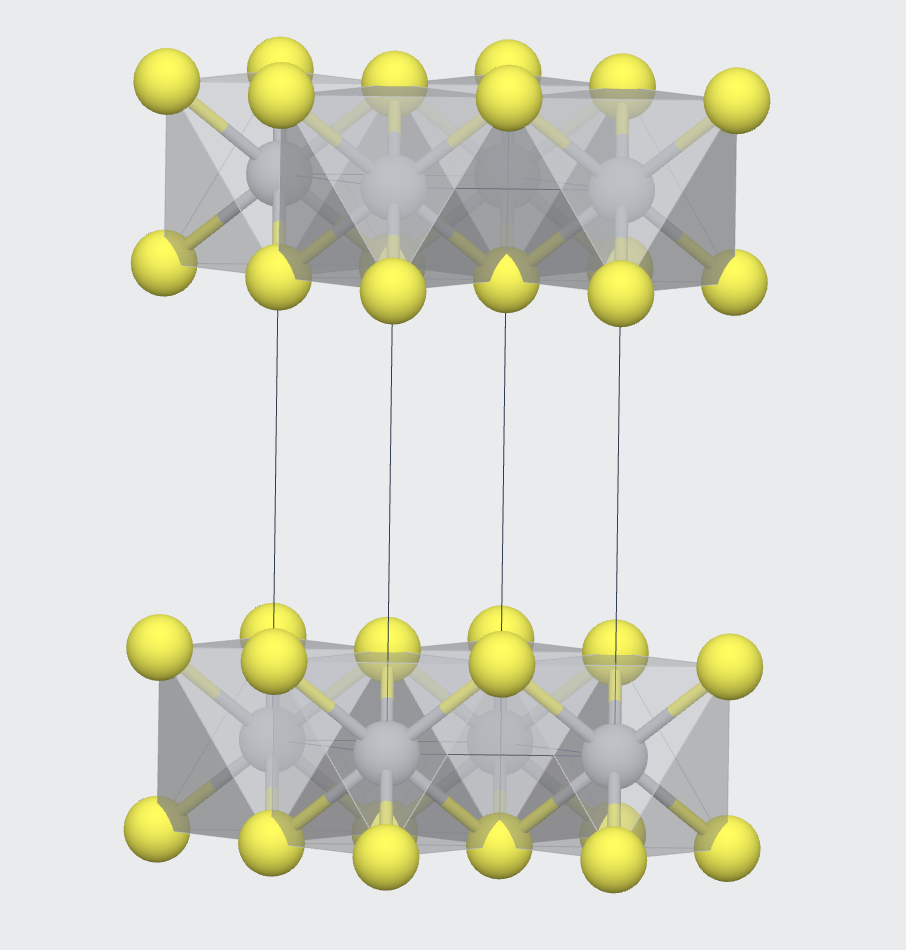
\includegraphics[width=0.5\textwidth]{TiS2.png}
    \caption{The two-dimensional structure of $\ce{TiS_2}$. From a slight angle along the b-axis. The titanium in \textcolor{gray}{grey}, sulfur, in \textcolor{yellow}{\textbf{yellow}}. Lithium-ions would intercalate into the space between the $\ce{TiS_2}$ layers \cite{materialsproject:TiS2}.}
    \label{fig:MPTiS2}
\end{figure}

The layered structure of these type of electrodes allow their reversible behavior. In 1980 John B. Goodenough introduced $\ce{LiCoO_2}$ (\ac{LCO}) as the cathode material for lithium batteries. This earned him together with M. Stanley Whittingham and Akira Yoshino the Nobel Prize in Chemistry in 2019 \cite{nobprize}. Goodenough and colleagues obtained a current density of up to $\SI{4}{mAcm^{-2}}$ \cite{mizushima1980lixcoo2} \cite{goodenough1980solid}. Even though the properties where exceptionally good at the time, the batteries were still not commercialized due to metallic lithium being too unstable, ergo an unsafe anode material. This was due to dendrites growing out of the anode that short circuited the battery. 

In 1991 Sony introduced lithium batteries, with LCO as the cathode, on the commercial market. LCO compounds provide good electrical performance, are relatively safe, easy to prepare, and are not especially sensitive to process variation and moisture. The metallic lithium anode was substituted for graphite which reduced the growth of dendrites at the anode. The electrolyte was an organic solvent with a lithium salt. 

A lithium-ion battery refers to a battery where lithium intercalates in both electrode materials, both the cathode and the anode. Lithium batteries, instead have an anode of metallic lithium. This nomenclature is transferable to other type of batteries like magnesium-ion/magnesium batteries. 

Figure \ref{fig:LiCoO2} shows a typical lithium-ion battery with $\ce{LiCoO_2}$ as the cathode and graphite as the anode. During discharge the lithium-ions move from the anode, through the electrolyte and separator to the cathode. The electrons move from the anode to the cathode through a separate external circuit, where the electrical energy can be extracted. When charged an over-potential is applied and the reaction is reversed. The overall reaction is shown in equation: (\ref{eq:LiB})

\begin{figure}[H]
    \centering
    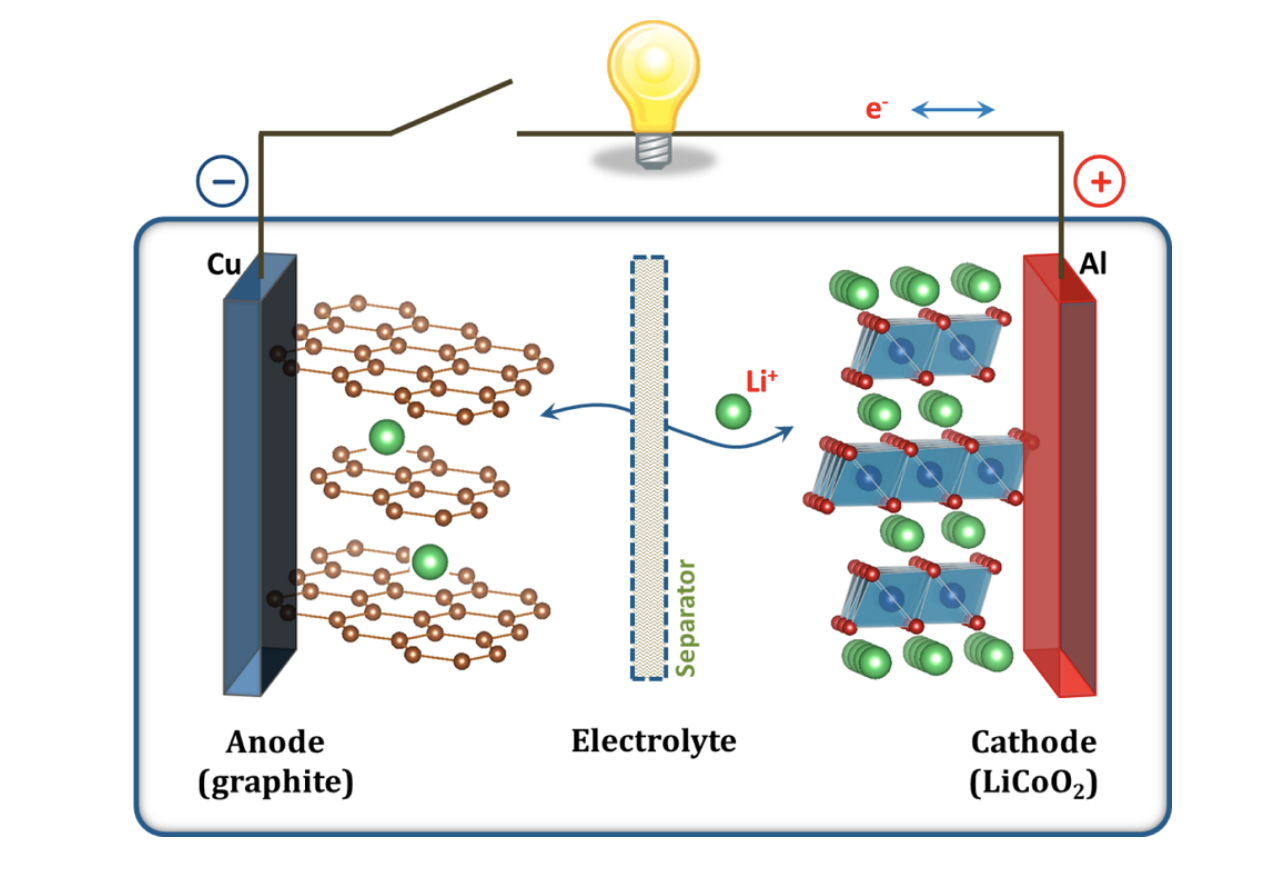
\includegraphics[width=0.8\textwidth]{Li-ion_inter.png}
    \caption{Schematic illustration of the first Li-ion battery $\ce{LiCoO_2/Li^+}$ electrolyte/graphite \cite{goodenough2013li}.}
    \label{fig:LiCoO2}
\end{figure}

\begin{align}\label{eq:LiB}
\ce{LiCoO_2} + \ce{C_6} \rightarrow \ce{Li_{1-x}CoO_2} + \ce{Li_xC_6}
\end{align}

The cathode materials used in lithium-ion batteries have evolved since the 1990s. Typical cathode materials, as of today, are $\ce{LiMn_2O_4}$ (spinel) and $\ce{LiFePO_4}$. $\ce{LiMn_2O_4}$ is a good ionic conductor due to the structure having channels in all three dimensions where lithium can be transported \ref{fig:LiMnO2}. $\ce{LiFePO_4}$ has the lower ionic conductivity of the two, due to only having channels in one dimension, as shown in figure \ref{fig:LiFePO4}. Even with a lower ionic conductivity, it is still a popular material due to its long cycle life. 

\begin{figure}[H]
    \centering
    \begin{subfigure}{0.30\textwidth}
        \centering
        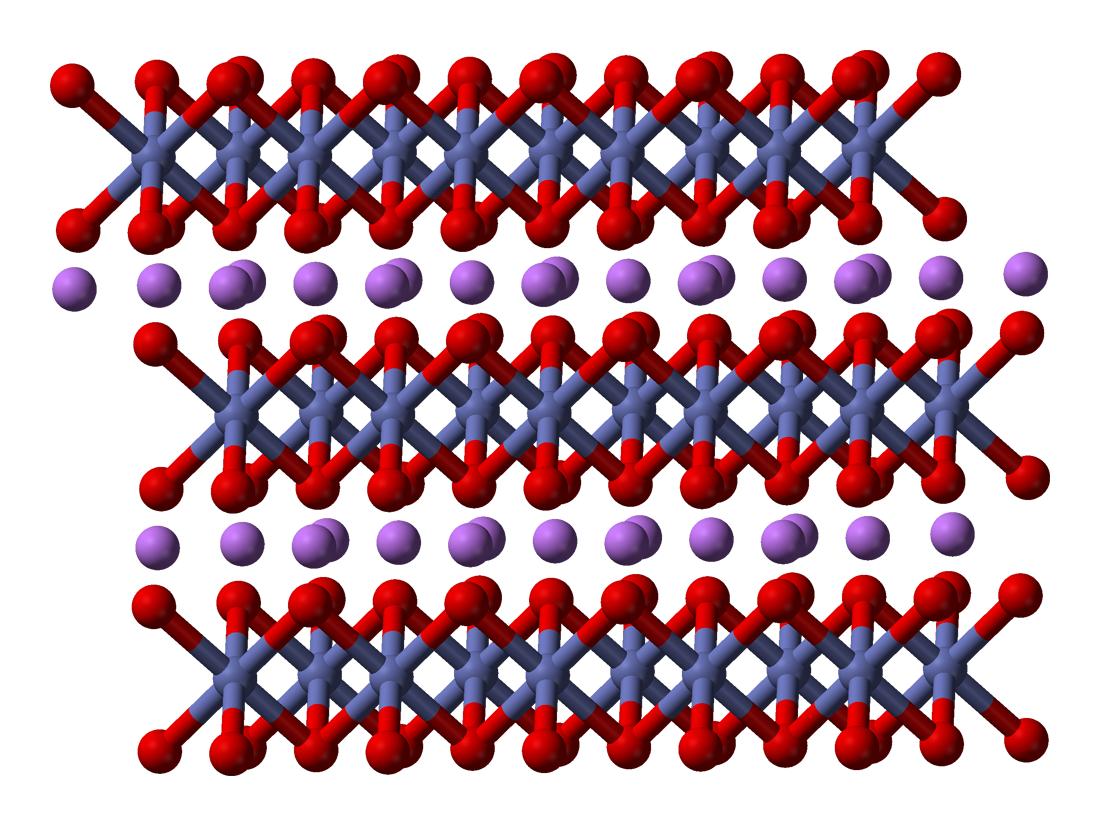
\includegraphics[width=\linewidth]{Lithium-cobalt-oxide-3D-balls.png}
        \caption{}
        \label{fig:LiCoO2_pic}
    \end{subfigure}%
    ~ 
    \begin{subfigure}{0.36\textwidth}
        \centering
        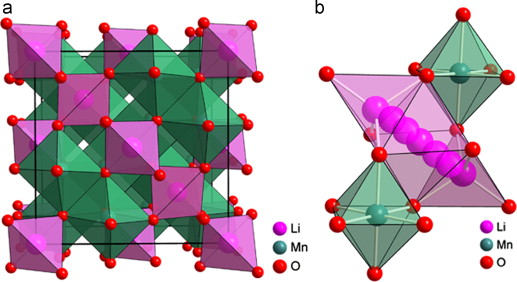
\includegraphics[width=\linewidth]{a-Crystalline-structure-of-spinel-LiMn2O4-and-b-its-corresponding-lithium-diffusion}
         \caption{}
         \label{fig:LiMnO2}
    \end{subfigure}
    ~ 
        \begin{subfigure}{0.30\textwidth}
        \centering
        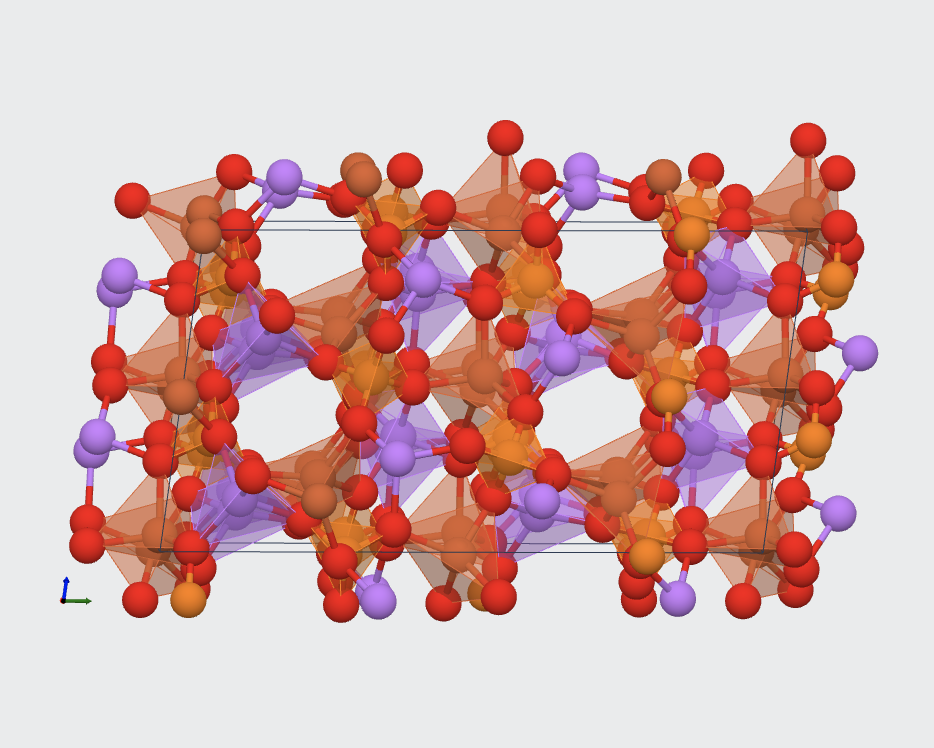
\includegraphics[width=\linewidth]{LiFePO4.png}
        \caption{}
        \label{fig:LiFePO4}
    \end{subfigure}
	\caption{Crystal structures of the layers in a) $\ce{LiCoO_2}, $ \cite{wiki:LiCoO2} b) the 3-dimensional channels in $\ce{LiMn_2O_4}$ \cite{zhang2013understanding}, c) and the 2-dimensional channels in $\ce{LiFePO_4}$ \cite{materialsproject:LiFePO4} are illustrated.}
	\label{fig:Li_a-c}
\end{figure}

The most used anode materials for lithium-ion batteries are graphite and other forms of carbon based materials. Graphite has a high energy density, making the cathode material the limiting factor for energy density of Lithium-ion batteries. The improvement of the cathode material is therefore high in priority among many research groups. Another recent anode materials is $\ce{Li_{4/3}Ti_{5/4}O_4}$ spinel, which has a lower specific capacity than graphite, but has a longer cycle life and good thermal stability characteristics. Nanostructured $\ce{Sn-Co-C}$ alloys commercialized in 2005 by Sony and Si-based negative electrodes seem promising for Li-ion cells with higher specific energy and energy density.

The main reasons for the use of Li-ion batteries can be summarized as follows: They have a long shelf and cycle life, low self discharge rate, high energy efficiency, high energy density, high rate and power discharge capabilities, no memory effect and many possible chemistries offer design flexibility. While some common drawbacks are: moderate initial cost, degeneration when discharged below $\SI{2}{V}$, degradation at high temperature (above $65^{\circ}\si{C}$ they can permanently lose capacity), their need for protective circuitry, capacity loss and potential for thermal runaway when overcharged and when crushed. Some also become unsafe if rapidly charged at sub zero temperatures.

For more than 40 years, the search for batteries with efficient energy storage, high capacity, long cycling and shelf life has been necessary to satisfy our demands for cheap, transportable power. Lithium batteries using lithium metal anode have attracted attention due to their promises of high energy storage capacity. However the batteries are prone to dendrites when plated, which results in short circuit and fire hazards \cite{xu2004nonaqueous}\cite{kim2013metallic}, Many possible solutions are being proposed \cite{liu2016lithium} \cite{zhang2015ex} \cite{li2018self} \cite{lee2017suppressing}. In recent years a desire to move towards an ultimate energy density technology has forced researchers to evaluate technologies beyond Li-ion batteries, where other metals such as magnesium and aluminum are pointed out \cite{reddy2011linden} \cite{yoo2013mg}. Aluminum and magnesium are considered because of their abundance. In the case of aluminum it has a high theoretical voltage, a high specific energy, and it is the most abundant metal in the world. It is hindered by a oxide layer on its surface \cite{li2002aluminum}, but solutions to this problem is being offered for large-scale applications \cite{van2014rechargeable}. Aluminum-based batteries are outside the scope of this work and will not be discussed.


There is also an ongoing search for candidates for solid-state electrolytes, due to energy density and safety being the main factors that govern the development of the rechargeable battery technology \cite{guzik2019lightweight}. Solid-state electrolytes would enable stable and reliable operation of all-solid-state Li-, Na-, and Mg-based batteries. Special focus is given to lightweight complex metal hydrides, due to their high ionic conductivity, and in some cases electrochemical properties that enable battery reversibility. 


%----------------------------------------------------------------------
\subsection{Magnesium based batteries}
	
	Magnesium batteries have been used as a primary battery, but historically, there has been little interest due to hydrogen gas generation during discharge, and relatively poor storage-ability of partly discharged cells. When fully charged the storage-ability, even under high temperature, is good \cite{reddy2011linden}, which has made the battery relevant for military application. 

	Recently magnesium batteries have attracted increased attention due to Mg higher volumetric capacity than lithium (i.e. $3832 \si{mAh cm^{-3}}$ vs $2061 \si{mAh cm^{-3}}$). Being the fifth most abundant element \cite{muldoon2012electrolyte}, makes magnesium, with its low atomic weight, low cost, and electrochemically active nature, a good candidate for battery applications. It can serve as a possible negative electrode with its electrochemical potential of $\SI{-2.37}{V}$, and it is environmentally friendly. 

	 While not competitive with Li metal on both specific capacity ($2205\text{ } \si{mAh g^{-1}}$ vs $3862\text{ } \si{mAh g^{-1}}$) and redox potential ($700\text{ }\si{mV}$ lower), dendrite formation is absent, which alleviates the safety concerns \cite{aurbach2003nonaqueous}. Still, there are several roadblocks ahead when looking at the possible electrolytes. One is the unique electrochemistry which prohibits its reversible deposition in aprotic solvents contained in commercial ionic salts such as magnesium bisimide or magnesium perchlorate. Magnesiums low reduction potential gives it a tendency to form surface films  that hinder ionic conductivity, opposite to Li compounds who also creates surface films, but these being ionic conductors and behaving like solid electrolyte interfaces. This not being the case for Mg compounds which creates blocking surface layer that inhibits deposition and conduction of magnesium ions \cite{aurbach2001comparison} \cite{gnanaraj2003improving}.
	
	There is an ongoing search for high performance cathode magnesium materials for the realization of a practical, rechargeable Mg battery. The $\ce{Mg^2+}$ shows promises of a instant multiplication of the electrical energy that can be released for the same volume, but the strong interaction between the $\ce{Mg^2+}$ ions and the host create problems \cite{van2014rechargeable}. This have lead to a search for electrodes and electrolytes that will allow the double charged magnesium ions to move through the host more easily. It is almost two decades since the first secondary magnesium battery was made, but these batteries are still at the research stage \cite{attias2019anode}.
 


%----------------------------------------------------------------------

%"The most advantageous combination of cathode and anode materials are those that will be lightest and give a high cell voltage and capacity. \cite{reddy2011linden}"\\
%Some of the most important properties in an anode are; Hight coulombic output(Ah/g), good conductivity, stability. \\¨
%Lithium is the lightest metal with a high value of electrochemical equivalence. With the development of intercalation electrodes, lithiated carbons are finding wide use. Lithium alloys are also being explored for use as anodes in lithium-ion battery.\\
%The cathode must be a good oxidizing agent, be stable, when in contact with a electrolyte, and have a useful working voltage.

\subsection{Cell operation principles and design}
Batteries are electrochemical devices. They store chemical energy that can be converted into electrical energy. This is done by an oxidation-reduction (redox) reaction where one of the species in the reaction gains or loses an electron by changing the oxidation number.  One battery consists of one or more \textit{cells}. A cell is fundamentally made of three parts; the anode, the cathode, and the electrolyte.
The anode is a negative electrode, which refers to the direction of current through the electrode. It is commonly a metal that would oxidize if given the opportunity. For a conventional current flow the electron moves from the anode to the cathode. The anode is often low voltage.  
The cathode is a positive electrode. The cathode is a metal that is normally combined with oxygen and is where the reduction occurs. A common example of a oxide is iron oxide. The cathode is normally high voltage. 
The electrolyte is the material that, when introduced to the anode and the cathode, provides an electrically conducting medium for transfer of charge. Electrolytes are typically liquid, to impart the ionic conductivity. It can be a solid, but this is, at least for now, less common. The cell will produce electricity when the circuit is complete. The electrolyte can, in some designs, act as both electrolyte and anode or cathode. 

If the anode is made from pure metal and has an external cathode of ambient air it is referred to as a metal-air electrochemical cell. These batteries have a much higher theoretical energy density. However there are technical issues confronting their development. \cite{li2017metal} 

The difference between high- and low voltage is referred to as the cell voltage, which is the driving force for the discharge of the battery. For secondary batteries, it is possible to recharge batteries by reversing this process by applying an external electrical power source, it creates an over-potential, i.e. a higher voltage than the one produced by the cell, with the same polarity. 

Changes in the design of the cell dictates the cells performance. If the compositions of the electrodes are altered, the cell will yield a different amount of electricity. Adjustments in the cell can affect the amount of electricity, the rate of production, the voltage, and the cell's ability to function in different temperatures. There is almost an endless amount of possibilities, even though the most common cell has been $1.5$ volt alkaline batteries. Other types of batteries include Lithium  batteries, Magnesium batteries, Zinc batteries,  Mercury batteries and others.

%\subsubsection{The manufacturing process of an Alkaline battery}
%In alkaline batteries the cathode is used both as the container and the cathode. Manganese dioxide, graphite, and the electrolyte are mixed and ganulated and pressed into hollow cylinders called reforms. The performs can be stacked or replaced by an extruded ring of the same material. The performs are then combined with nickel-plated steal. These are then the containers of the battery. 

%A separator is then soaked in the electrolyte solution and inserted between the cathode and where the anode is supposed to be. The anode is then put into the can, it is a gel composed of zinc powder and other materials like potassium hydroxide electrolyte. The gel does not fill the whole can, so that there is room for the chemical reaction to occur. 

%The can is then sealed with three connected components. The first being a current collector, going to thirds of the way trough the anode with a plastic seal at the top before it is all closed by a metal cover with a metal cap. The current collector goes all the way through the plastic seal and is connected to the metal cap. The seal is thinner in some places, in case of gas build ups. In some battery designs, wax are used instead of a plastic seal, so excessive gas can push through the wall. Lastly a label is attached to the battery, with the necessary information about the battery. 

%The battery is then taken through a complex quality control, to certify the batteries ability to resist corrosion, maintain a good shelf life, usage life, and other factors. 




\subsection{General introduction to battery properties}\label{sec:msp}
	
	In a cell there are essentially two areas, or sites, in the device where the redox reactions occur. In general these half-cell reactions can be expressed as one reduction and one oxidation reaction:
	
	$$\text{aA} + ne \leftrightharpoons \text{cC} $$
	
	Where a is the number of molecules of substance A taken up by $n$ electrons to form c  molecules of C, and the oxidation reaction defined in the same way:
	
	$$\text{bB} \leftrightharpoons \text{dD} + ne $$ 
	
	with the overall reaction, as exemplified by the Daniell cell  \ref{eq:Daniell} being: 
	
	\begin{equation}
	\text{aA} + \text{bB} \leftrightharpoons \text{cC} + \text{dD}
	\label{eq:redox}
	\end{equation}
	
	
	Whenever there is a reaction there is a decrease in the free energy of the system.  This is free energy is called standard Gibbs energy and it is defined as:  
	
	$$\Delta G^0 = -nFE^0$$
	
	Where $n$ is the number of electrons in the reaction, and $F$ is the Faraday constant ($F = 96485\text{ }\si{C mol^{-1}}$). Gibbs free energy of the reaction is the driving force of the battery and enables it to deliver energy to an external circuit. $E^0$ is the standard potential of the cell. It is determined by the type of active material in the cell, i.e. the difference in electrode potential between the cathode and anode. $E$ decides how easy it is to remove one electron from a atom. It can be calculated from the free energy or from the standard electrode potential \ref{eq:standard_potential}. 
	
\begin{align}\label{eq:standard_potential}	
\text{oxidation potential} + \text{reduction potential} = \text{standard potential}
\end{align}
	e.g. from our database:	
	\begin{align}
	\ce{Li^+(aq)} + e^- \rightarrow \ce{Li (s)} &  & \SI{-3.04}{V}\\
	\ce{Bi^{3+}} + \ce{3e^-} \leftrightharpoons \ce{Bi(s)} &  & \SI{0.317}{V} \\
		& &  E^0 =  \SI{3.357}{V}
 	\end{align}
	
	Direct measurements of the absolute electrode potential is difficult to achieve, so a reference point is defined. The standard potential of \ce{H_2 / H^+} is set to zero and all other standard potentials are compared to this potential. If to metals are interconnected in a electro chemical cell, the metal with the larger standard reduction potential will gain electrons. A rule of thumb is, from low to high, alkali metals, alkaline earth metals, aluminum, base metals (e.g. $\ce{Fe}, \ce{Ni}$), hydrogen, and transition metals. 
	
	In situations where the system is not in the standard state, the \textit{voltage} $E$ of a cell is given by the Nernst equation.
	
	\begin{align} 
	E = E^0 -\frac{RT}{nF} \ln{\frac{a^c_C a^d_D} {a^a_A a^b_B} } 
	\end{align} 	
	where $a_i$ is the activity of the species. $R$ is the gas constant, and $T$ is the absolute temperature.  
	
	The \textbf{voltage} can be defined as the difference between two electrical potentials. In most batteries the electrical potential difference occurs due to the redox reaction in the electrodes that creates a potential gap between the electrode and the electrolyte. When an outer circuit is connected this gap is lowered, but due to the reaction rates going up, the potential gap is maintained.
	
%	In this work we will refer to the \textit{Average Voltage} (\ac{AV}) of the battery, that is, the average voltage during discharged. It is lower then the 
	
	\textbf{Capacity} is a measurement of how much charge a battery can hold. It is most common to evaluate the capacity of an electrode or a battery in terms of capacity per weight $\si{mAh/g}$, i.e. the gravimetric capacity (\ac{GC}). It can also be denoted as capacity per volume $\si{mAh/m^{-3}}$, i.e. the volumetric capacity (\ac{VC}). The capacity of a battery is often compared to the theoretical capacity which is determined by the amount of active material in the cell. It can be found by Faraday's law \ref{eq:faradays_law}. 
	
	\begin{align}\label{eq:faradays_law}
	Q=\frac{mFz}{M}
	\end{align}
	
	Where $F$ is Faraday's constant ($F = 96485\text{ }\si{C mol^{-1}}$), $z$ is the valence number of ions of the substance, $m$ is the mass and $M$ is the molar mass of the substance in grams per mol. 
	
	Capacity can also be defined as:
	\begin{equation}
	C = \int I(t)\cdot dt
	\end{equation}
	
	Where $i$ is the number of electrons or cations exchanged between the negative and positive electrodes, i.e. how much charge a battery can store. $I(t)$ is the current, the number of electrons flowing over the external circuit per time interval $dt$, which is integrated over the discharge period. Theoretically, capacity is $1$ gram equivalent weights of the active material (in grams) divided by the number of electrons in the reaction.	
 

	If the calculations are based on only the active materials participating in the electrochemical reaction the theoretical capacity of a $\ce{Zn/Cl_2}$ cell is $2.54\text{} \si{g/Ah}$ or $0.394\text{} \si{Ah/g}$.
	

	\begin{align}
	\ce{Ze} + \ce{Cl_2} &\rightarrow \ce{ZnCl_2}\\
	1.22\text{ } \si{g/Ah} + 1.32\text{ } \si{g/Ah} &= 2.54\text{ } \si{g/Ah}
	\end{align}
	
	Notably, when calculating the theoretical capacity of a battery it is higher than the actual capacity. This is due to the mass of the electrolyte, separator, and other battery components that is missing from the equation.
	
	The active materials of the electrodes allow the reversible uptake and release of ions. This may happen by movement of the ions in a couple of different ways. They can move into their chemical structure through intercalation, or they can move out of their chemical structure, through extraction or deintercalation. Lastly, this can also be done by conversion of the electrode material into other more ion rich/poor chemical forms or mixtures. 
	
	The total Li or Mg content in the electrodes will either be varied by changing the composition of one phase or the ratio between coexisting phases. In this work we will only look at intercalation type batteries, as will be discussed. 
		
The voltage of a battery determines the work a battery can do and depends on the types of active materials used. The cell voltage is also limited by concentration and temperatures, as expressed by the Nernst equation. A higher voltage is desirable, because of the increase in work that can be done by the battery.

The calculation of the voltage of a lithium ion battery is more complex than calculating the voltage of a common electrochemical cell with two electrodes in a wet solution. The voltage of an electrochemical cell is calculated from the difference in chemical potential for the lithium on the anode and the cathode \cite{aydinol1997first}, as shown in eq\ref{eq:V_OC}.

\begin{align}\label{eq:V_OC}
V_{OC} = \frac{\mu_A - \mu_C}{F}
\end{align}

Where F is Faraday's constant and $\mu_A$ is the chemical potential of the lithium anode, and $\mu_C$ is the chemical potential of the lithium cathode. The cell potential is thus decided by both the difference in electronic potential and the lithium ions movement. The energy from the electronic potential is calculated from the redox potential of the lithium cathode and anode, while the energy from the ion movement is dictated by the crystal structure and the coordinates of where the lithium ions were intercalated or deintercalated.  

\textbf{Energy density} (\ac{ED}) is related to the capacity of a battery. The energy density of a material is the energy of a system per volume ($\si{mWh/g^{-1}}$). Another closely related term is specific energy (\ac{SE}), which is the energy per unit mass ($\si{J/kg}$). The formula for energy density is given in equation \ref{eq:ED}
	
	\begin{align}\label{eq:ED}
	P = Q \cdot U
	\end{align}

Where $P$ is the efficiency or energy density of the material. $Q$ is the capacity of the material, and U is its potential. We can calculate the energy density for a battery with $\ce{LiCoO_2}$  as the cathode and a graphite  anode ( while ignoring the rest of the battery) as shown in equation \ref{eq:EDc}, assuming a average voltage of $\SI{3.6}{V}$. 

\begin{align}\label{eq:EDc}
P = 100\text{ }\si{mAhg^{-1}} \cdot \SI{3.6}{V}  = 360 \text{ } \si{mWhg^{-1}}
\end{align} 

This is the theoretical energy density of a battery with LCO as the cathode and graphite as the anode. The specific energy density, i.e. where the battery is included in the calculations in its entirety, of the same composition results in a energy density of $190\text{ } \si{mWhg^{-1}}$ \cite{srinivasan2008batteries}.  
	
 	Capacity and energy densities of battery materials can be compared relative to mass, volume and cost. The more electrode material that a battery contains, the greater is its capacity and energy. The higher the cell voltage the greater its power and energy. 
	

Some relations important for this work are the relation between energy, energy density, capacity, power and current. These relate to each other as shown in equation \ref{eq:battery-properties}, where $E$ is the energy ($\si{Wh}$), $V$ is the voltage ($\si{V}$), $C$ is the capacity ($\si{Ah}$), $U$ is the energy density ($\si{J/m^3}$), $P$ is the power ($\si{W}$), $I$ is the current ($\si{A}$) and $t$ is the time ($\si{h}$)

\begin{align}\label{eq:battery-properties}
V \cdot C &= E \\
\frac{E}{Volume} &= U  \\
V \cdot I &= P \\
W \cdot t &= E 
\end{align}




	Energy is the cells ability to do work, which is a property of high interest for practical applications. 
		
	The battery can deliver power which is defined as:
	\begin{equation}
	P(t)=V(t)I(t)
	\end{equation}
	Where $I(t)$ is defined as earlier, and drawn at a cell voltage $V(t)$. The amount of work that can be done by the battery or the energy contained in the battery, is then defined as the power delivered over the discharge period.
	
	\begin{equation}
	W = \int P(t) \cdot dt = \int V(t)I(t) \cdot dt
	\end{equation}
	
	This is particularly interesting for applications that require a lot of work in a short time period.	

\subsection{Cell definitions used in this work }\label{sec:theory_bat}
In this thesis, especially under the section on general properties of battery, terms related to features used from Materials Project database are used. These terms will be defined or clarified here.

	The features discussed here are based on optimal design and discharge conditions. These values are helpful to set a number on the "goodness" of a battery. The actual performance may vary under normal conditions of use. 
	

	\textit{Energy} is the computed energy, it is the total energy or sum of the electronic energy and nuclear repulsion energy. 
	
	\textit{Energy per atom} is the computed energy normalized per atom in the unit cell.
	
	The \textit{formation energy per atom} is calculated from the formation energy from the elements normalized per atom in the unit cell.

	
	\textit{Volume} is the volume of the unit cell.
	
	\textit{Band gap} is the distance between the valence band and the conduction band, it represents the minimum energy that is required to excite an electron up to a state in the conduction band. In general, band gaps computed with common exchange-correlation functionals such as the LDA \cite{perdew1983physical} and GGA are severely underestimated \cite{perdew1985density}. Typically the disagreement is reported in luterature to be $\tilde 50\%$. Internal testing by the Material Project supports these statements; reporting band gaps underestimated by $\tilde40\%$. 
	

	
	\textit{Density}, here defined as the calculated bulk crystalline density. Typically underestimated due to the calculated cell volume being overestimated on average by $3\% (\frac{+}{-} 6\%)$ \cite{jain2011high}.

	
\textit{Magnetic moment} ($\si{\mu_B}$) is calculated for the unit cell within the provided magnetic ordering. 
	
	\textit{Number of sites} is the total number of atoms in the unit cell. 
	
	\textit{Elasticity} is the predictor associated with the elastic properties of a solid, i.e. the elastic constant. It provides a complete description of the response of the material to external stresses in the elastic limit \cite{de2015charting}. 
	
	
	\textit{Polarizability} is a tabulated atomic properties. It is the ability to form instantaneous  dipoles, and is defined as: 
	
	\begin{align}
	\alpha = \frac{P}{E}
	\end{align}
	
	Where $\alpha $ is the polarizability in isotropic media, $p$ is the induced dipole moment of an atom to the electric field $E$ that, is the field that produces the dipole momentum. 
	
	\textit{Van der waals volume} ($V_W$) of a molecule are the space occupied by the individual atom, which is impenetrable to other molecules at ordinary temperatures. For a single atom, it is the volume of a sphere with a radius equal to its van der Waals radius ($r_W$):
	
	\begin{align}
	V_W = \frac{4}{3} \pi r^3_W
	\end{align}
	

% 	\textit{Average Voltage} as we use, is defined as the voltage average during discharge. It is lower then the theoretical voltage.

% \subsection{Electrodes and features}
%	In this section the features used in ML as predictors will be introduces. First will the pair properties be introduced, before going into the more electrode specific features. 

	

%	\subsubsection*{Physical stability}
	 \textit{Physical stability} is the energy above hull in $\si{eV}$. It is the energy that is demanded for decomposition of the material into the set of most stable materials at that chemical composition. Positive values indicate that the material is not stable. While a zero energy above hull indicates that this is the most stable material at its composition. Stability is tested against all potential chemical combinations that result in the material's composition. For example a $\ce{Mg_3Sb_2}$ structure would be tested against other $\ce{Mg_3Sb_2}$ structures, against $\ce{Mg}$ and $\ce{Sb}$ mixtures, and against $\ce{MgSb}$ and $\ce{Sb_2}$ mixtures. 
	
	In a battery, the reactant is supplied from the electrolyte phase to the catalytic electrode surface. Electrodes are often composites made of active reactants, binders and fillers. To minimize the energy loss of both activation and concentration polarizations at the electrode surface and to increase the electrode efficiency, it is often preferred to have a large electrode surface area. This can be done by having a porous electrode design. A porous design can provide an interfacial area per unit volume that is considerable higher than that of a planar electrode. 
	
	A \textit{porous electrode} is an electrode that consists of porous matrix of solids and void space. The electrolyte penetrates the void space of a porous matrix. In such an active porous mass, the mass transfer condition in conjunction with the electrochemical reaction occurring at the interface is very complicated. In a given time during cell operation, the rate of reaction within the pores may vary significantly depending on the location. The distribution of current density within the porous electrode depends on the physical structure (pore size), the conductivity of the solid matrix and the electrolyte, and the electrochemical kinetic parameters of the electrochemical processes.  
	



		



%\subsection{Battery chemistries}
\begin{comment}
\subsection{Intercalation batteries and why Li}
The current Li-ion batteries offer some of the best combination of high specific energy, energy density, long cycle life and high-power capability, among the rechargeable battery technologies. They have dominate the worldwide market in portable and consumer electronic equipment, electric vehicles, space applications, as well as electrical energy storage. Li-ion batteries have minimal side reactions when a Li ion intercalates into the cathode/anode materials. They exhibit limited self-discharge, and no memory effects that limit energy density after many cycles. Their energy efficiency may be further enhanced by lowering the internal resistance of the battery, and Li-ion batteries as a result, receive considerable attention at both fundamental and applied research levels.


The development of stable novel materials is the key to the successful development of novel and advanced rechargeable batteries. Current research and development has focused on upgrading the energy density of Li-ion batteries. 

Most practical
rechargeable batteries deliver capacities and energy densities
far below their theoretical values(med kilder)due to limited utilization
efficiency of the active materials that participate in electrochemical reactions. The major reasons for such limitations
include effects that result from slow electrode process kinetics
with high polarization and low ionic diffusion or electronic
conductivity rates, particularly at the electrolyte–electrode interfaces. Material stability issues caused by a low Li content can
also impact on its degree of charging. Therefore, the improvement
in existing rechargeable battery systems involves exploring key
materials and focusing our attention on the atomic, ionic, or
molecular diffusion and transport. Charge transfer, the optimization of surface and interface structure, and the regulation of
electrochemical reactions within Li-ion systems may pave the
way for improved (i) capacity, and energy and power density,
(ii) reactivity, reversibility, and structural stability during charge–
discharge cycles, (iii) ionic diffusion and electronic transfer at
high charge–discharge rate, and (iv) lower cost, increased safety
and environmental compatibility


inkluder litt om dette? og med bilder kanskje?

The schematic diagram of the current Li-ion battery based on
a carbon based anode (LixC6), cathode (LiCoO2), liquid electrolyte (LiPF6 dissolved in a mixture of EC and DMC or equivalent),
and separator is shown in Fig. 2.9 In the foreseeable future,
Li-ion batteries will be the most practical solution to a wide
range of electrical energy storage applications.10


. The majority new cathode
materials for Li-ion batteries under research and development
are transition metal oxides, which tend to provide lower discharge
potential as the electric-capacity density increases. Carbon-based
materials (usually graphite) are currently used as anode materials
in Li-ion batteries. The other variety of carbon-based materials and
pure Li metal are currently proposed as alternate anode materials,
but many need further improvement with respect to electrode
potential and charge–discharge cycle life concerns

"\cite{bhatt2015recent}

Working principle of Li-ion cell. 

When a Li-ion battery discharges, a $\ce{Li^+}$ moves from the anode (i.e. graphite) to the cathode (i.e. \ce{LiMO_2} where $\ce{M}$ is a transition metal), through the electrolyte that commonly is  $\ce{Li^+}$ -containing salt. The reaction, as discussed above \ref{eq:redox}, are:


$$\ce{LiMO_2} \leftrightharpoons   \ce{Li_{1-x}MO_2} + \ce{xLi^+} + \ce {xe^-}\text{ (cathode)} $$
$$\ce{xLi+} + \ce{xe^-} + \ce{xC_6} \leftrightharpoons  \ce{xLiC_6} \text{ (anode)} $$
The overall reaction:
$$\ce{LiMO_2} + \ce{6C} \leftrightharpoons  \ce{Li_{1-x}MO_2} +  \ce{xLiC_6}$$

The anode is graphite, thus there is noe metallic $\ce{Li}$, which makes the Li-ion battery less reactive, therefor safer, and the graphite anode offers a longer cycle life than their Li-metal counterpart. To progress the performance of Li-ion batteries a few design changes are needed; A cathode with a chemical potential that matches the electrolytes highest occupied molecular orbital, and an anode matching the lowest unoccupied molecular orbital of the electrolyte. A non-aqueous electrolyte of high $\ce{Li^+} $ ion conductivity under practical temperatures. 
\end{comment}



%\subsection{Mg- and Li- batteries: State-of-the-art}
	
	
	
\pagebreak
\section{Machine Learning}

In this chapter we introduce and summarize machine learning and related concepts. The first section introduces the basic ideas behind machine learning and one of the best known examples will be presented. Secondly the concepts of supervised and unsupervised learning will be presented with a clarification regarding the difference between regression and classification problems, so that we can discuss where this work resides in the field of machine learning. The basics of methods utilized in this work will then be introduced, emphasizing Random Forest. Subsequently a short description of the validation methods used is given. These are; K-fold cross validation and how it is used in optimizing our Random Forest method, root mean square error (RMSE) and R-squared($R^2$).
   
We conclude this section with a brief explanation on the role of data, how features can affect the effectiveness of a model, of the concepts of over- and under-fitting, and how these are related to the bias-variance-trade-off. 


\myworries{Sondre: Did you forget something? Come back to this when done with the section.}


\subsection{The Basics of Machine Learning}

Machine learning comes from the field of pattern recognition and learning theory, and is defined as the field of study that gives computers the ability to learn without being explicitly programmed. Or more precise: "… A computer program is said to learn from experience E with respect to some class of tasks T and performance measure P, if its performance at tasks in T, as measured by P, improves with the experience E…"(\cite{mitchell1997machine}). At its core the ability to learn by detecting patterns in usually huge amounts of data that, more often then not, is impossible to perceive for a human. 


	\subsubsection{The basics}\label{sec:introexample}
	As an introduction on how machine learning was applied to learn and recognize patterns in our work, it will be useful to start with a simple example applied to the recognition of the handwritten number "5". 
	

	How two people writes a single digit may vary to an extensive degree. It might seem to be a easy problem, but if the recognition is to be done manually million of times, it is no longer a trivial task for any human being. Therefore a model which can recognize these digits would be useful. A model that takes a picture of a digit as input and outputs that digit in a way that is recognizable for a machine, i.e. a digital format.
	
	Machine learning only works when you have data, preferably a large amount of data. For instance data from the MNIST test dataset \cite{lecun1998gradient}. This database contain $60,000$ images of handwritten numbers that is commonly used for both various training, and testing in the field of machine learning. The images all are 18x18 pixels. The data is divided into two sets, one training set: $X_{Train}$ and one test set: $X_{test}$. Some numbers from the MNIST database are shown in figure \ref{fig:MNIST}. 
	
\begin{figure}[ht]
    \centering
    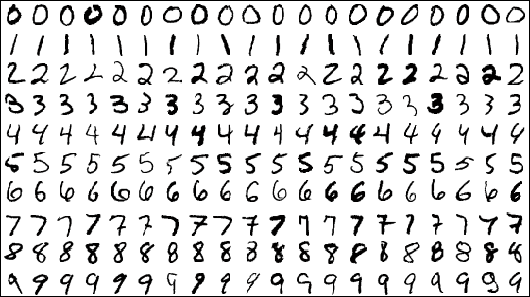
\includegraphics[width=0.8\textwidth]{theory/figures/MNIST.png}
    \caption{Number from the MNIST database \cite{MNIST}}
    \label{fig:MNIST}
\end{figure}
	
	How do one represent an image as something that makes logical sense to a computer? Most learning algorithms take numbers as input. To a computer one image a grid of numbers that represent how dark a pixel is. So each picture contains a gray-scale value that ranges from $0$ to $255$. Where each sample can be viewed as a vector consisting of 324 \textit{features}. Every sample has a corresponding label value, or \textit{target}, which is the digital equivalent to the handwritten sample. We let the corresponding targets be denoted: $y_{train}$ and $y_{test}$, for training and testing data. Next we designate our \textit{learner} denoted by function $h$. $h$ is then given our training set $S$, where $S = (X_{train1}, y_{train2}),..., (X_{trainN}, y_{trainN})$ and returns a prediction rule: $h: X \rightarrow y$. This rule is also called a predictor, in general, a classifier, or a regressor, depending on the problem in question. 
	
	The \textit{training phase} is a process where the learning algorithm gets tweaked to best capture the correlating structure of the data set, so that it can better predict new data. As mentioned in the last paragraph the output from the \textit{training phase} is called a \textit{predictor}. The next step is to introduce the \textit{predictor} for new, unseen data, so that it can be classified. Then we compare the $y_{test}$ to our predicted value $y_{pred}$ given by $h$ to see if our model generalizes well to unseen data in $X_{test}$. 
	
	\subsubsection{Supervised and Unsupervised Learning }
	One of the most basic separations in machine learning is the partition between supervised learning and unsupervised learning \cite{gentle2012handbook}.
	
	In the case of supervised learning, the answer to a problem is known and given to the computer. The computer then deduce its own logic to figure out how to get to that result, thus the name complete-date problem is commonly used. This is the most common type of learning. With unsupervised learning the machine is tasked with finding patterns and relationships in data sets without any prior knowledge of the system, incomplete-data problems. Some authors operate with a third and a forth category, namely reinforcement learning, where the machine learns by trial-and-error, and evolutionary learning, where they account for the biological evolution and that it can be seen as a learning process \cite{marsland2014machine}.
		
	In this thesis, only supervised learning is considered. Algorithms and challenges specifically related to unsupervised learning, reinforcement learning, and evolutionary learning, is therefore not further examined. 

	\subsubsection{Regression and Classification Problems}
		A response variable can either be qualitative or quantitative in nature. For the qualitative response variable, let's assume a set of data points $ \vec{x}$ and a goal of finding the value of the output $y$ when $x = 0.5$. The value $x $ is not in the data points given so a way to \textit{predict} the value, is needed. Given in the example above, we assume that there exists a function $h$ that the value comes from. When that function is found one can find any given $y$ for any given $x$. This is what is known as a regression problem - The response variable takes form of a continuous numerical value. The regression problem is a problem of function approximation or interpolation. It may occur a scenario where there are multiple functions, lets say $h$ and $g$, that fits the given data perfectly. If this is the case one value in-between the data points is selected, and both the functions, $h$ and $g$, tries to predict its values and the results are compared to see which is better.
	This does not seems as very intelligent behavior, but the problems of interpolation can be very difficult in higher dimensional space. This can also be observed in classification, the other aspect of what our algorithms can do.  
	
	If the response variable is quantitative the problem is referred to as a classification problem. Such a problem consists of taking several input vectors and deciding which of $N$ classes they belong to. This decision or prediction comes from training on examples of each class. To be clear, classification problems are of a discrete nature - The input only belongs to one class, like the example given at the start of this section \ref{sec:introexample}.
	
	In this work we want to predict characteristics of batteries, these properties have continuous values, meaning that the task at hand is a regression problem.
	
	\subsubsection{Data collection, Preparation, Features and Feature Selection}
	 
	Normally the data collection is a large part of the work and not easily available, or, at the very least, needs to be assembled and prepared. If the problem is completely new it might be natural to engulf this step with the next one. (Which is, more or less, what this work tries to do.) With a small dataset with many different features one can experiment and try to figure out what features are the most useful before picking those and collecting a full dataset based on them and then perform a complete analysis. 
	
	A common problem in similar studies is that there are too many types of data that can be relevant, but that data is hard to find or represent in a way that makes sense for the machine. This can be because it requires too many measurements, or, something that is prevalent in this work, that they are in a variety of places and formats. For instance; if the measurements are already taken, but at vastly different temperatures they might be hard to compare or merge. It is important to have a \textit{clean} dataset, this means that the dataset does not have missing data, significant errors, and so on. On top of all of this, supervised learning requires a target $y$, which demands time and involvement of experts. 
	
	The specific input to a model is normally referred to as a feature, that is, numerical representation of raw data. The amount of features are of importance for the machine learning algorithm to successfully make a good prediction. If there are to few relevant features one can not make an accurate prediction due to the lack of necessary data. And if there are to many features, or many of the features are irrelevant to the task the model will be more expensive.
	
	The amount of information needed is extensive, and should be of high quality. A bigger dataset demands a higher cost, and predicting the amount of data required is a futile endeavor. Luckily Machine Learning is still less computationally costly than modeling full systems at a micro or nanoscale, which makes it interesting in the field of material science. 
	
	
\subsection{Bias-variance tradeoff}\label{sec:Bias-variance tradeoff}

As the algorithm learns we need to make sure that it generalizes well to data not in its training set. Obviously the algorithm can not generalize beyond the limits of the training data. Therefore it is important to minimize the two sources of errors known as \textit{bias} and \textit{variance}. This is know as the \textit{bias-variance trade off}. It is the property of trying to minimize the two errors simultaneously, and should not be confused with the \textit{irreducible error} of a model which is a result of the noise of the data. These three together are the terms used to analyze an algorithms expected \textit{generalization error}, which is a measurement of how accurately an algorithm is able to predict outcome vales for unseen data.    


Our machine is bias if it generalizes too much. The error is due to low variability in our training data, or that it did not adapt to the training data appropriately. The machine misses the relevant relations in the data set between the features and the output. This effect leads to that which is commonly referred to as under-fitting, see left on figure \ref{fig:bias_var}. 

Variance is the error that stems from high variability, and the degrees of variability in most machine learning algorithms is large \cite{marsland2014machine}. In simple terms, there is a low degree of generalization. It might be a perfect fit, but as soon as new data are introduced the predictions plummet. This is commonly referred to as over-fitting, see right on figure \ref{fig:bias_var}. 

\begin{figure}[h]
     \centering
     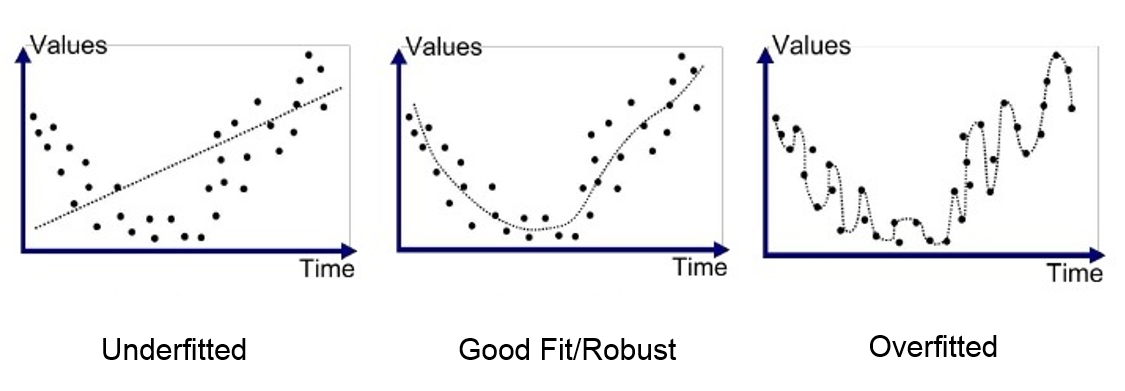
\includegraphics[width=\linewidth]{theory/figures/Bias_variance.png}
     \caption{Simplified illustration showing the concepts of bias-variance problem. Left to right; high bias, low bias and low variance, high variance \ref{fig:bias_var}}.
     \label{fig:bias_var}
\end{figure}

A good way to understand the idea of the bias-variance tradeoff is, a more complex model with an increased number of features is not necessarily better at predicting what you want to predict. 


\subsection{Random Forest}

\subsubsection{Ensemble learning}
	There are many different machine learning algorithms, in this work we have focused on the \textit{ensemble method}; \textit{Random Forest} \cite{breiman2001random}. The idea of ensemble learning is that two heads are better than one, so why not have many learners that all get slightly different results on the same data, and then combine them, as shown in figure \ref{fig:ensemble_learning}.
	
\begin{figure}[h]
     \centering
     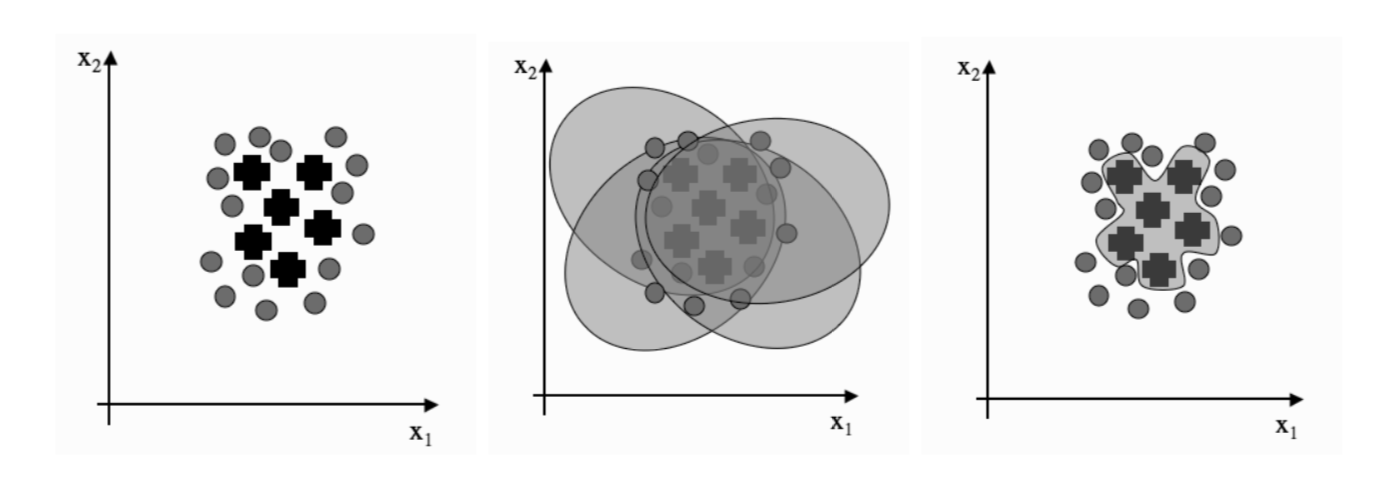
\includegraphics[width=\linewidth]{theory/figures/ensemble_learning.png}
     \caption{Combining different classifiers trained on the same data, which in combination can make a much better decision boundary on the target data. Adopted from \cite{marsland2014machine}}
     \label{fig:ensemble_learning}
\end{figure}	

Ensemble methods are particularly useful in machine learning when there is little data, as well as when there are to much data, this is heavily due to cross-validation, which will be explained later \ref{sec:cross_validation}). 

\subsubsection{Decision tree}

A decision tree is a low cost binary flowchart-like structure. It is one of the most common data structures in the field of computational science, both because of the low cost to make the tree, but also because the cost of using the tree is even lower; $\mathcal{O}(\log{N})$, where N is the number of data points \cite{marsland2014machine}. 

Decision trees are structured much like a regular tree \ref{fig:decision_tree}, at the top there is a base, or a \textit{root}, down the branches there are chance nodes, and at the end of the branches there are \textit{leaves}, or end nodes. Every internal node is structured like an conditional statement on a feature.

Let us say that you want to play tennis. You look out the window, and there are three possible weather states (root node); rain, overcast or sun. If it is overcast you will play either way, but if it is windy, you need to evaluate if that wind is strong or weak (chance node). If it is little wind, you will play. Else, it is strong and you will not play (end nodes). 

The chance nodes are the results from these tests, and the leaves are the class labels. The full route from root to leaf is the classification rule, or \textit{branch}. An advantage of Random Forest being based in decision trees is that the algorithm is much more like a "white box" compared to Neural networks "black box" approach, because we can retrace the decisions of each tree. This is especially helpful in the research done in this work where we want to figure out the roll of every feature, and how they affect the result.

\begin{figure}[h]
\centering
\begin{tikzpicture}
  [
    grow                    = right,
    sibling distance        = 6em,
    level distance          = 10em,
    edge from parent/.style = {draw, -latex},
    every node/.style       = {font=\footnotesize},
    sloped
  ]
  \node [root] {Outlook}  
    child { node [dummy] {Humidity}
      child { node  [env] {No} 
        edge from parent node [below] {High}}
	  child  { node  [env] {Yes}  
	  edge from parent node [below] {Normal}}
	  edge from parent node [below]{Sunny?}}
%  --------------------------------------------------------  
    child { node [env] {Yes}
      edge from parent node [below] {Overcast?} }
%  --------------------------------------------------------    
    child { node [dummy] {Wind}
      child { node  [env] {No} 
        edge from parent node [below] {Strong}}
	  child  { node  [env] {Yes}  
	  edge from parent node [below] {Weak}}
	  edge from parent node [below]{Rain?}};
\end{tikzpicture}
\caption{A simple example of a decision tree for playing tennis. Root in red, leaf node in blue.}
\label{fig:decision_tree}
\end{figure}
\subsubsection{Random Forest}
Random Forest (\ac{RF}) is a ensemble learning method, the idea is that one decision tree is good and many trees, or a forest, is better. The most interesting part of Random Forest is the randomness that is introduces. Several classifiers are achieved by using the simple combination method \textit{bagging}. Bagging stands for \textit{bootstrap} aggregating. Bootstrapping is the process of taking a sample from the original dataset at random, and replacing parts of it with other original data, so that it is not equal to the original data. There will then be several samples where some of the data is equal, while others are completely different. For bootstrapping in Random Forest, one sample is taken from the dataset for each tree. 

A new parameter is then introduced, at each node a random subset of features are given to the tree, it can only make decisions based on that specific subset, and not the original tree. This increases the randomness in the creation of each tree, and it speeds up the learning process. The reason to add randomness to the algorithm is to reduce variance without effecting bias. It also removes the need for decision tree \textit{pruning}, i.e. reducing the complexity of decision tree by removing the parts of the tree that does not help the classifier and it reduces overfitting. The process of creating trees is repeated until the error stops decreasing. 

When the forest is done, we use a majority vote system, which is a comparison of the mean response for regression. For a step by step algorithm, see the README.txt file on \href{https://github.com/sondrt/Machine-Learning-the-Voltage-Capacity-and-Energy-density-of-Electrode-Materials}{github}. 
The reason for not using cross-validation in the learning algorithm, which is common in other machine learning methods \ref{sec:cross_validation}, is that our bootstrap method only uses about $65\%$ of the data, leaving $35\%$ on average which can give a estimated test error. 

The main reason we decided to opt in for Random Forest is due to an article by \cite{fernandez2014we} and the findings from both our collaborators \cite{tsamardinos2020automated} and Shandiz and colleagues \cite{shandiz2016application}, that clearly state that Random Forest is the chosen machine learning algorithm when you want to test for correlations. Another reason and a main advantages of RF is that it is fast and does not require any particular optimization of its hyper-parameters (e.g. number of decision trees for RF). On the other hand, methods like support vector regression (SVR) require an extensive search for the optimum hyper-parameters before providing reasonable results.

%\subsection{Support Vector Regression}
%	Dette bør brukes og kan da skrives om.
%	\subsubsection{Radial Basis Function Kernel}
%	\subsubsection{SVR and the Bias-Variance-Trade-off}
	
	

\subsection{Evaluation method}\label{sec:evaluation_method} %Mean square error, Root mean square deviation and Mean absolute error, Weighted absolute percentage error}
%In this section different evaluation methods used in the work will be explained. 
%These are Mean square error, Root mean square deviation, Mean absolute error, Weighted absolute percentage error, The Coefficient of Determination, k-fold cross validation.


\subsubsection{Mean and Variance}
One of the most recognized properties of a distribution is its \textit{mean}, or expected value. It is denoted by $\mu$, and defined as: $E[X] = \sum_{x \in \chi}x p(x)$, for discrete variables.

The variance is a measure of the "spread" of a distribution, denoted as $\sigma^2$. It is defined as:

\begin{align}
\text{var}[X^2] = E[(X - \mu)^2]
\end{align}

from which:

\begin{align}
E[X] =\mu^2 + \sigma^2
\end{align}

can be derived. For a ML model, a prediction is done with an accuracy $x_acc$ on training data and its prediction accuracy on test data is $y$ then: 
\begin{align}
\text{var} = x_{acc} - y
\end{align}

\subsubsection{Standard deviation}

Standard deviation (\ac{std}) is a tool to quantify the measure of spread. It is very similar to variance by yielding the measure of deviation whereas variance provides the squared value. Standard deviation is defined as:

\begin{align}
std[X] = \sqrt{var[X]}
\end{align}

 or:

\begin{align}
std = \sqrt{\frac{\sum^N_{i=1} (x_i- \hat{x})^2}{N-1}}
\end{align}

\subsubsection{Mean square error} 
 
The Mean Square Error (\ac{MSE}) can give a measure of the quality of our estimator \cite{robert2014machine}. It is defined as
\begin{equation}\label{eq: mse}
	\text{MSE}(\epsilon) = \frac{1}{n}\sum_n^{n-1}\epsilon^2 = \frac{1}{n_\text{samples}} \sum_n^{n_{\text{samples}}-1}(y_i - \hat{y_i})^2
	\end{equation}
	Where $\hat{y_i}$ is the predicted value of the $i$-th sample, and $y_i$ is the corresponding true value.
As such it can be thought of  as the average of the square of our residuals. Therefore the MSE can never have negative values, and smaller values mean that we have a better prediction, where at zero there is a perfect fit.

\subsubsection{Root mean square deviation} 
The Root mean square deviation, or root mean square Error (\ac{RMSE}), is defined as the square root of the MSE:
$$\text{RMSE} = \sqrt{\text{MSE}} =  \sqrt{\frac{\sum^{n-1}_{n}(y_{i}-\hat{y_{i}})^2 }{n}} $$
And is thus the distance, on average, of a data point from the fitted line, measured along a vertical line. The RSME is directly interpretable in terms of measurement units, and is therefore a better measure of goodness of fit than a correlation coefficient. 

RMSE and Stdev can seem very similar, but they are not the same. Stdev measures the spread of data around the mean, while RMSE measure distance between some values and predictions for those values. If the mean error approaches $0$ and n approaches infinity Stdev and RMSE converge. 

\subsubsection{Mean absolute error}
Mean absolute error (\ac{MAE}) is another statistical tool that is used to measure the difference between two continuous variables, in our case; the predicted values and the observed values. It corresponds to the expected values of the absolute error loss. The MAE is defined as:

\begin{align}\label{eq:MAE}
\text{MAE} = \frac{1}{n_{samples}}\sum^{n_{samples}-1}_{i=0}\abs{y_i - \hat{y_i}}
\end{align}

where $y_i$ and $\hat{y_i}$ are defined as above. In geometrical terms, it is the average absolute vertical/horizontal distance between each point in a scatter plot and the $Y=X$ line. 

\subsubsection{Weighted absolute percentage error}

Weighted absolute percentage error (\ac{WAPE}) is the mean absolute error divided by the mean ($\bar{y_i}$) multiplied by a hundred. This yields the mean error in percentage. 

\begin{align}\label{eq:WAPE}
\text{WAPE} = \frac{\text{MAE}}{\bar{y}_{i}} \cross 100 
\end{align}
 


\subsubsection{$R^2$ score - The Coefficient of Determination}

	In regression validation the $R^2$ is the standard when it comes to measuring goodness of fit \cite{james2013introduction}. In straight terms it is the proportion of the variance in the dependent variable that is predictable from the independent variable.

\begin{equation}\label{eq: R squared}
	R^2 =1 - \frac{SS_{res}}{SS_{tot}} =  1 - \frac{ \sum(y_i-f_i)^2 }{ \sum(y_i-\bar{y}_i)^2 }
\end{equation}

	Where $y_i$ are the indexed response variables (data  to be fitted) and $f_i$ the predictor variables from the model with $\epsilon_i = y_i - f_i$. The average of the response variables is denoted $\bar{y}_i$. The second term can also be considered as the ratio of MSE to the variance (the $1/n$ factors null each other out in a fraction), or the total sum of squares ($\ac{SS}_{tot}$). 
	
	If the residual sum of squares ($SS_{res}$) is low the fit is good. However, this should be compared to the spread of the response variables. After all, if the response variables are all nicely distributed close to the mean, then getting a good $SS_{res}$ is not suspicious. We therefore do a normalization in the fraction, taking the scale of data into consideration. In the simplest polynomial fit, using a zero order polynomial (a constant), our model would just be a constant function of the mean. The sums being equal, returning unity on the fraction and the total $R^2$ score would be zero. In the other extreme, if the model fits perfectly, than $SS_{res}$ would be zero and the $R^2$ score would be one. In this sense we have a span of possible $R^2$ scores between zero and one, from the baseline of the simplest model at zero, and a perfect fit at one. In contradiction to most scores the value can be negative, because the model can get arbitrarily worse, thus giving negative values.
	The $R^2$ score is useful as a measure of how good our model is at predicting future samples.
	 
\subsubsection{K-fold cross validation}\label{sec:cross_validation}
	K-folding is a cross validation technique that allows us to generalize the trends in our data set to an independent data set. In this way we can circumvent typical problems like over-fitting and selection bias \cite{james2013introduction}. The approach for the technique is simple and represented in figure \ref{fig:cross-validation}. Instead of doing a regression on the entire data set, it is first segmented into $k$ number of subsets, or splits, of equal size (making sure to pick out the variables randomly before distributing them to the subsets). 
	
	Now one subset can be chosen to be the 'test' or 'validation' set while the rest of the subsets ($k-1$ of the folds) are the training sets. The desirable regression is then applied on the training set, arriving at some data fitting that is the prediction. From here it is a straight forward process to analyze how well our predicted variables compare to the validation variables, e.g. through the $R^2$ score function. However, even though the subsets are picked randomly, the validation subset used could potentially not be a representative selection of the entire set. Therefore the process is repeated $k$ times, each time using a new subset as the validation subset. Finally, one can simply calculate the average of the scores to get the predictive power of our model. As an added benefit, since the calculations are done anyways, the average of the predictions can be used as the final fit. 
	
	Cross validation techniques are very useful when the gathering of new data is difficult or impossible, as we are using the extra computational power at our disposal to squeeze the most amount of relevant information out of our data. 

\begin{figure}[h]
    \centering
    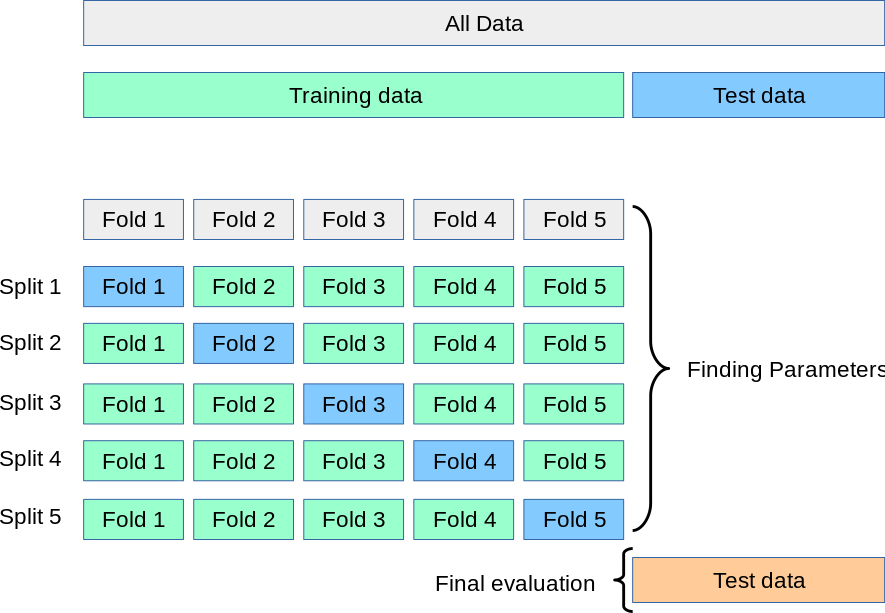
\includegraphics[width=0.8\textwidth]{theory/figures/grid_search_cross_validation.png}
    \caption{A representation of how cross-validation is done. First the data is split into $K$ number of sets, then one of these sets are left out as test data. The model trains on the training data before being tested on the test data. This process is repeated $K$ times, and the mean is taken \cite{fig:cross_validation}.}
    \label{fig:cross-validation}
\end{figure}

\FloatBarrier
\subsection{Principal Component Analysis }\label{sec:PCA}
	Principal Component Analysis (\ac{PCA}) \cite{james2013introduction} is a procedure that uses orthogonal linear transformation to reduce the amount of feature subspaces. It goes under different names in different fields, but the most recognizable might be Single Value Decomposition. It consists in converting a set of possible correlated variables into a set of uncorrelated variables, called principal components (\ac{PC}s). 
	
	The PCs are arrayed so that the first PC has the largest variance, meaning that it accounts for the largest possible amount of variability in the dataset. The second PC does the same, it accounts for as much variability as possible with the constraint of being orthogonal to all the former components. These orthogonal vectors are linear combinations of an uncorrelated orthogonal basis set. Graphically, the shortest vectors affect the predictions the least. Since PCA is sensitive to the relative scaling of the original variables, in \textit{sklearn.decomposition.PCA}, (the library we use), the input data are centered but not scaled, before performing the PCA.
	
	Figure \ref{fig:PCA} shows, the training data from the Mg-db plotted in two scatter plots. To the left is our original data uniformly scaled, scaled so that the variance is equal to one, the mean of the distribution is zero, and about $68\%$ of the values lies between $-1$ and $1$. To the right, a plot showing the affine transformation of these data (PCA), which have been translated, rotated and uniformly scaled. As can be seen in figure \ref{fig:PCA_b}, this affine transformation leads to clearly distinguishable classes.

\begin{figure}[h]
    \centering
    \begin{subfigure}{0.48\textwidth}
        \centering
        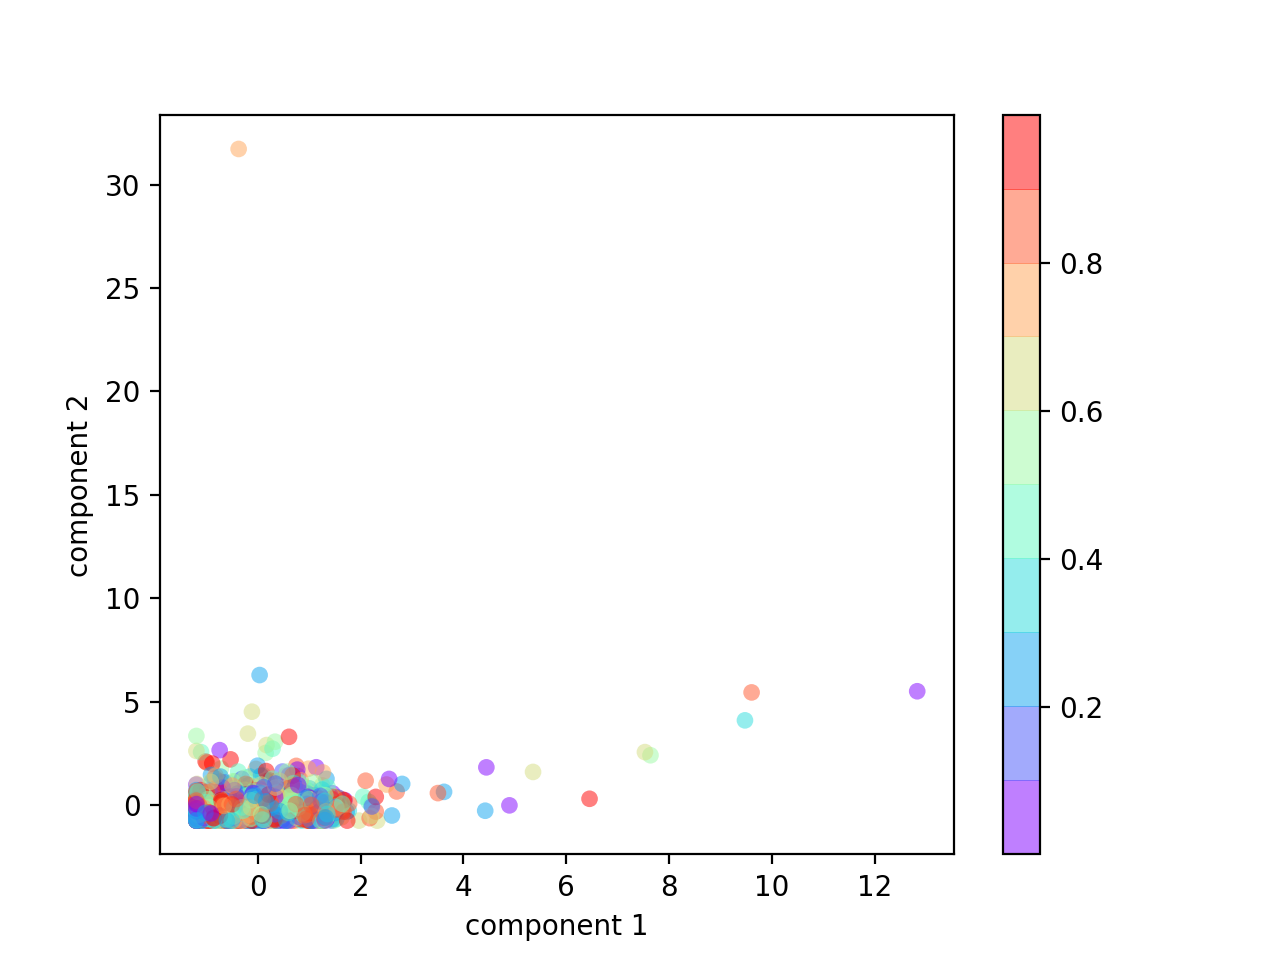
\includegraphics[width=\linewidth]{theory/figures/standardscalar_bpca.png}
        \caption{}
        \label{fig:PCA_a}
    \end{subfigure}%
    ~ 
        \begin{subfigure}{0.48\textwidth}
        \centering
        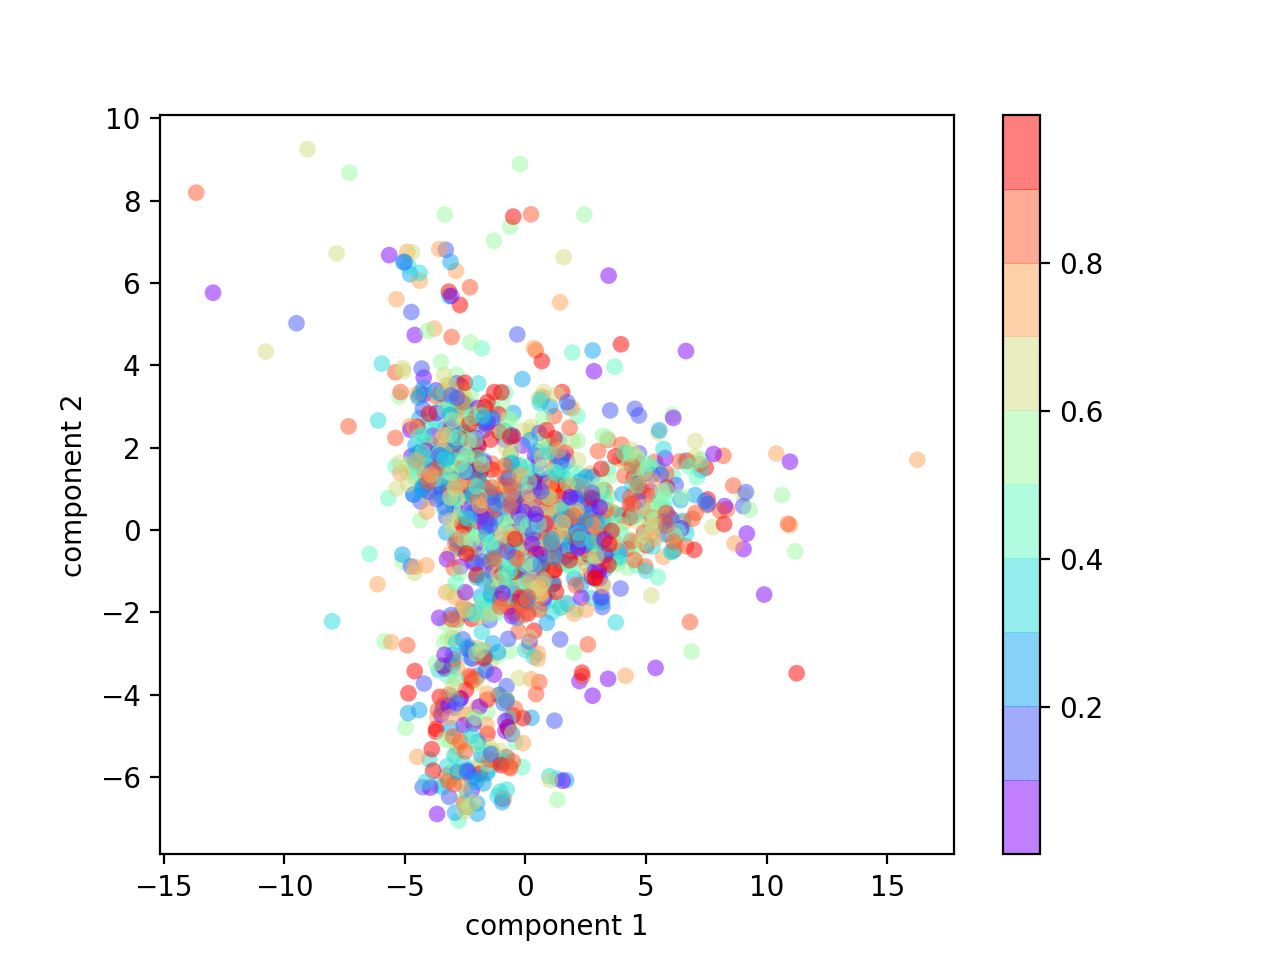
\includegraphics[width=\linewidth]{theory/figures/standardscalar_apca.png}
        \caption{}
        \label{fig:PCA_b}
    \end{subfigure}
	\caption{Two scatter plots; On the left, some of our data from the Mg-ion database before PCA. On the right, our data after PCA, showing that there are distinguishable classes.}
	\label{fig:PCA}
\end{figure}
%\subsection{Mutual Information**}
%Ranking of features. 
%This can be useful.
%\subsection{Machine Learning $\cross$ batteries}
\subsection{Earlier work}

The field of material science is blooming due to computing power being cheaper and more available than ever before. When the Human genome project started in the 1990 the main problem was lack of computational power, but because of Moore's law, the sequencing of all 3 billion letters of DNA is not even a challenge in todays computational standard. In the field of material science, researchers have known how to simulate materials since the early 1900, due to the discovery of quantum mechanics, the challenges are related to the of computational power.

An advanced material have an order of $10^{23}$ electrons that demands computational methods to simplify the problem \cite{electromaterials}. The gap between the computation needed and what state-of-the-art systems are providing is increasing \cite{reddy2011linden}.

In the field of computational material design a subfield called 'high-throughput' (\ac{HT}) computational material science is on the rise \cite{potyrailo2011combinatorial} \cite{pang2020additive}. This area is based on computational quantum - mechanical - thermodynamic approaches, and a multitude of techniques both in database construction and in the field of intelligent data mining. The idea is simple; first construct a large enough database of accurate thermodynamic and electronic properties of existing and hypothesized materials. Secondly, use different algorithms and statistical models to intelligently analyze the data and find materials with desired properties. This method should continuously be validated by comparing the calculated values with real  (already known) materials, and later also on new hypothetical materials, to create a feedback loop to further improve the algorithm \cite{curtarolo2013high}. To simplify, a computational HT method consists of three tightly connected steps: Virtual material growth, rational material storage, and material characterizations and selection. This work is based on the second and third step, rational material storage and material characterization and selection, on intercalation type batteries.

Several studies on batteries have applied machine learning and different degrees of HT, in particular to estimate their state of charge accurately and to improve their energy system management  \cite{kalawoun2015novel} \cite{chemali2018state} \cite{hu2015battery} \cite{ermon2013learning}.
	In the direction of predicting battery properties only a handful of studies were found. Shandiz \textit{et al.} \cite{shandiz2016application} used classification methods to determine the crystal system of silicate cathodes. They found that the Random Forest classifier gave the highest accuracy of prediction, and that there is a strong correlation between the three major crystal system (monoclinic, orthorhombic and triclinic), and other features of cathodes. Their data was taken from the online database Materials project \cite{Jain2013} \cite{Zhou2004a} \cite{Adams2011a}.
	Sendek and \textit{et al.} \cite{sendek2017holistic}, constructed a classification model using logistic regression to find possible solid state electrolytes for lithium-ion batteries. They concluded that simple atomistic descriptors alone, were not enough to obtain useful predictions. Instead, using a multi-descriptor model can yield good predictions.
	Similar to this work Joshi \textit{et al.} \cite{joshi2019machine} employed ML techniques to predict electrode voltage for metal-ion batteries from the Materials Project database. Much like this thesis, their emphasis were on finding proper features vectors that could accurately represent the compounds.

%The idea of using higher valence cations such as magnesium or aluminum, which could increase capacity while at the same time reducing weight and volume, had not yet been considered in computational studies, in 2013. 
Other areas where ML have shown promise are in the field of Nanoporous Materials \cite{fanourgakis2019robust}. Three a set of new descriptors for predictions on methane adsorption was proposed. Fanourgakis \textit{et al.} combined structural features, such as the helium void fraction, surface area, and pore volume, with other descriptors designed, such as the probe atoms of various sizes on MOFS. The work lead to a more general application of ML on nanoporous materials \cite{fanourgakis2020universal}. It was found that introducing "atom types" as descriptors in the ML algorithm to account for chemical character of both the MOFs and the Covalent Organic Frameworks (COFs) improved the ML predictions significantly. 


\pagebreak
\part{Method}
\section{Method: Better section header}
	In this section we will introduce the overall approach to the research. First introducing the data set and experimental environment, before going through technicalities in the methods used to represent physical and chemical properties of the electrode materials.

	The two most crucial challenges in ML are; Create the dataset, which needs to be big enough and as accurate as possible to better the predictions given the right features. Secondly, finding the right descriptors. If not both of these conditions are fulfilled, then it is not possible to create a reliable ML model. \myworries{Put in ML part?}
	
	All codes are written in Python 3.7 \cite{van1995python} or Fortran98 \cite{backus1964fortran} and can be found here: \url{https://github.com/sondrt/Creten_Stuff} \myworries{gitrep private, change?}. And all computations are done on a (give computer specifics.), if nothing else is noted \myworries{Any libraries that uses this? read machine architecture. }. The main frameworks and libraries we used for our data mining and data analysis are Python with NumPy \cite{oliphant2006guide}, JSON \cite{pezoa2016foundations}, Pandas \cite{mckinney-proc-scipy-2010}, and Scikit-learn \cite{scikit-learn}.
To make the AP-RDF files Fortran90 was used. 

\subsection{Data set and Experimental Environment}\label{sec:experimentalenv}
%Introduce the overall approach to the research. 

	 The techniques used in this work are the \textit{volumetric number density} (\ac{vnd}), the \textit{Void fraction} (\ac{vf}) and the \textit{atomic property weighted radial distribution function}(\ac{AP-RDF}). Other properties used where introduces in the foundation section \ref{sec:msp}. Lastly we quickly mentions the basics of our algorithm. 
%	Wanted to explore the possibility of using machine learning(ML) to predict different characteristics of batteries, based on their cathode and anode materials.
 

	 The first needed for this task was a database(\ac{db}), we found several, but opted into \textit{materialsproject} \cite{Jain2013} \cite{doi:10.1038/sdata.2015.9} (mp), due to their investment in the battery explorer (\url{www.materialsproject.org/batteries}) \cite{Zhou2004a} \cite{Adams2011a}, which made, the otherwise main task of this work, collecting the data, much easier, and a functioning API \cite{Ong_2015}. The db has a sizable amount of information on electrodes available. MP has $16128$ conversion electrode and $4401$ intercalation electrodes. We decided to limit the project to the intercalation electrodes, due to this limiting the variation of materials in the db. 
	 
	 First of all mp had the reduced cell formula with consistent CIF files for all voltage pairs, that is; both the charged and discharged material. Secondly many different characteristics or voltage pair properties are present. Some of these characteristics, that we used as targets in this work, are; Average voltage, Gravimetric and volumetric Capacity, Specific Energy $(\si{Wh/kg})$, Energy density $(\si{Wh/l} )$, and a measurement of the stability; energy above hull measured in  $\si{eV/atom}$. Other properties that where in the mp db and to some extent tested as predictors for each material, both charged, and discharged are; the space group, energy per atom, volume of the unit cell, volume change in percentage, band gap, density, total magnetization, number of sites, and elasticity. 

The database contains more than $4400$ intercalation electrodes, where we have used $2291$ Lithium-ion batteries, and $360$ Magnesium-ion batteries, for our analysis. This could easily be expanded to the $321$ Natrium-ion batteries, and $481$ Calcium-ion batteries in the db. With new compounds being added to the database continuously, including many new structural predictors, there is a high likelihood of an increase in accuracy over time, due to the db growing. Our method were tested on Mg-intercalation electrodes as well as Li-intercalation electrodes, then compared to each other to identify correlations on the valuableness of our predictors. 

	It is important to note that we have a minimum of two predictor per property of the material at any given run. This is due to how we defined each battery. They have at least one charged and one discharged state, and only one target(ref to theory machine learning). For any given property we have one value calculated for the charged material, and one for the discharged material.This means that we predict for a specific charged- or discharged half cell configuration.

	Exemplified by the battery $\ce{Mg(CrS_2)_2}$ with the battery ID: $mvc-1200000091$, it has two material ID's, one for the discharged- ($mvc-91$)\label{ex:MgCrS22-discharged}, and one for the charged($mvc-14769$) \label{ex:MgCrS22-charged} material. This pair will be referred to in this section. 
	
	The sum of features that uniquely represent each compound in the Li data set are $238$ and $177$ for the Mg data set. The feature vectors are vastly different and their numerical values ranges from the thousands down to small fractions. Therefor these were normalized for better prediction capability, for faster training of the model and to avoid any bias preference for a particular feature. The input was normalized to be between $-1$ and $1$, it were done while training our model, and the target values $y$ where not normalized. 


\subsection{Volumetric number density } \label{sec:volumetric_number_density}

	Volumetric number density, \textit{n}, is used to describe concentration of countable objects. And is defined as: 
	
\begin{equation}\label{eq:n}
n= \frac{\#\text{ of atoms}}{\text{Volume of the unit cell}}
\end{equation}

	Where \textit{Volume} is the volume of the unit cell. \myworries{write volume of unit cell in formula?}
	
	Technically, in the volumetric number density, there is a predictor for each individual element. That is; if the intercalation battery framework is $\ch{Mg(CrS_2)_2}$ then the the number density for; magnesium, chromium, and oxygen, related only to that material, will be predictors. The charged material will have the predictors with the values: $S_{vol} = 36.6292$ and $Cr_{vol} = 18.3150 $. While the discharged material will have the predictors with the values: $S_{vol-dis} = 30.1286$, $Cr_{vol-dis} =18.3150 $, and $Mg_{vol-dis} = 7.5321$. All other elements still exists as predictors for this framework, both charged and discharged, and exist as possible branches in the decision threes, but they are given the value $0$. This quality is uniq for the volumetric number density, and all other predictors minimize "empty" columns. 

It is probable that such a direct measurement of a geometrical aspect could be a good predictor due to the physical significants of the information. If RF were applied on to the entirety of the CIF file, it is probable that it would make a bad fit, due to the bias-Variance-trade-off as mentioned in section \ref{sec:Bias-variance tradeoff}, and because of the difference in complexity of some of these files. \myworries{ref to two vastly different files in the appendix or on github?}




\pagebreak
%--------------------------------------------------------------------------------
\subsection{Void Fraction} \label{sec:Void_Fraction}
\myworries{rewrite}

	Void Fraction, or the porosity, is a measurement of the void space in the material. Calculations are based on classical force fields that describe interatomic interactions between the atoms of the material and a helium atom. Poreblazer \cite{ongari2017accurate}. We measure the accessible void, that is, the total amount of free space in the material and it is a quantity that can be measured experimentally. 
			
	The pore volume is obtainable experimentally under the assumption that Gurvich rule is valid, it assumes that the density of the saturated nitrogen in the pores is equal to its liquid density, independent of the internal void network. 
%	It states that "if the density of the saturated nitrogen in the pores is assumed equal to its liquid density, regardless of the shape of the internal void network and, because of the weak interactions, regardless of the chemistry of the framework." 
and the pore volume ($v_{pore}$) and the porosity ($\theta$) can be  computed from:

\begin{equation}
v_{pore} = \frac{n^{ads,satd}_{N_2}}{\rho^{liq}_{N_2}}
\end{equation}
\begin{equation}
\theta = v_{pore} \cdot \rho_{cryst}
\end{equation} 

	Where $n^{ads,satd}_{N_2}$ is the specific amount of nitrogen adsorbed, $\rho^{liq}_{N_2}$ is the density of liquid nitrogen, and $\rho_{cryst}$ is the density of the crystal in question. It is important to understand that these experimental values does not account for all small voids between atoms where the nitrogen does not fit. There also exists pores that are non accessible for a nitrogen atom, so the experimental data using nitrogen is different form the DFT calculations using i.e. helium.

	There are many different computational method to obtain the pore volume where each one computes slightly different portions of the full volume. We have here used two approaches for measuring the pore volume. Frist, the geometric pore volume,$\text{Ge}_{pv}$, which is defined as all the free volume of the unit cell. Secondly helium pore volume ,$\text{He}_{pv}$, where the unit cell is probed with realistic intermolecular potential is tested. This makes the calculations temperature dependent. The calculation are done at $\SI{298}{K}$, more details on these calculations can be found in the file \href{https://github.com/sondrt/Creten_Stuff/blob/master/defaults.dat}{default.dat} in the supportive information/github.

	Void Fraction is a characterization method for microporous crystals and have had great success in metal organic frameworks (MOFS), as demonstrated also by the team of supervisors.
	
	In case of dens materials like the one we consider in this work, the void fraction should not be a good predictor. However we decided to include it in our tests in case the space occupied by the ion in the discharged material would impact our prediction, as will be discussed later. (REF)\myworries{rewrite.}


UFF \cite{rappe1992uff}

\subsection{AP-RDF Descriptors of Electrode materials}

	Atomic property weighted radial distribution function (AP-RDF)\ref{fernandez2013atomic} was found to be a good predictor which also, when tested by the PCA(REF to theory part), exhibited good discrimination of geometrical and other properties, in one of their cases, gas uptake.
	
	One of the methods found, that seemed to yield good predictions dependent on chemical properties where the Atomic property weighted radial distribution function, successfully used on MOFS. \ref{fernandez2013atomic} Due to it looking reasonable we decided to try it out.

	The radial Distribution Function(RDF) is the interatomic separation histogram representing the weighted probability of finding a pair of atoms separated by a given distance.(REF) In a crystalline solid, the RDF plot has an infinite number of sharp peaks where the separation and height are characteristic of the lattice structure. We used the minimum image convention (boundary condition)\myworries{Do I need a ref here?} and the RDF scores will be uniquely defined inside of the unit cell, per material-ID. The RDF can be expressed as:
\begin{equation}\label{eq:RDF}
RDF^P(R) = f \sum^{\text{all atom pairs}}_{i,j} P_i P_j e^{-B(r_{ij} - R)^2}
\end{equation}

In our case the RDF scores in a electrode framework has been interpreted as the weighted probability distribution to find a atom pair in a spherical volume of radius $R$ inside the unit cell according to equation above. \ref{eq:RDF}

Summing over all the atom pairs, where $R_{ij}$ is the minimum image convention distance of these pairs, $B$ is a smoothing parameter, and $F$ is a scaling or normalization factor. Our Own approach to this is written in Fortran, and can be found in the appendix with an operational pdf.(REF)

The RDF can be weighted to fit the requirements of the chemical information to be represented, by introducing the atomic properties, $P_i$ and $P_j$. We weighted the radial probabilities by three tabulated atomic properties namely electronegativity, polarizability, and Van der Waals volume, which gives us the AP-RDF. While a regular RDF function encodes geometric features, the atomic property weighted RDF additionally characterizes the chemical features within a material. An atomic property weighted RDF can be seen on the screen. 

To test our method, we used it to reproduce the results for the two MOFS, namely \textit{IRMOF-1} and \textit{MIL-45} found in the article by Fernandez.\ref{fernandez2013atomic}. We confirmed their findings .. though with drawback related to the size... which are flawed in our case.  In our opinion, we think that this is a fundamental drawback, and the results depends on the size of the simulation cell(which can be made by replicating the unit cell). 

INSERT BILDET AV PLOT AV AP-RDF. 

\subsection{Algorithm}

First of all, a wrote a program for "scraping" the \textit{materialsproject}webpage for batteries(0). This gave us the possibility to gather all the available resources on the batteries in the database in a fast and effective manor, as well as updating these CSV files of  battery-IDs. (ref)

We then run a second program that downloads all the information on the materials that matches a material-ID correlated to a battery-ID (1,2). (ref) Before constructing a CIF file structured so that all the battery-IDs, charged-material-IDs, and dischargerd-material-IDs are correlated with the information on the charged and discharged properties. 

After, the volumetric density fraction is calculated(3) and added to the main CSV file for both charged and discharged materials. While the CIF files are being processed for Poreblazer(4) where the void fraction is calculated(5,6). 

Then we merge all our CSV files based on what properties that we are interested in and makes a CSV file called for\_ML.csv(7,8) that we feed into our random forest algorithm(9). We then run cross validation, MSE, and plot what we are interested in(10).

In addition we also tested for different machine learning algorithms, as mentioned(ref), but these were only to test the reliability of our model, and will be discussed in the discussion section(ref) 





\begin{comment}
\myworries{This is in the intro.}
The original plan was to make a model that could predict Ionic conductivity for potential solid state electrolytes but after gathering and searching for information we found this article (REF:) by Sendek: Were they could not find a sufficient amount of data on ionic conductivity for a proper model to be created, or rather, they only found 40 materials that they used to make their prediction on ionic conductivity, something that our group deemed far to little for a proper prediction, even if we added the $ 40$ that we found from our own search. 

We then tried to use the materialsproject's database (MPDB), which resulted in a change of focus from electrolytes to electrodes, due to the nature of that database and ML's demand for as much relevant data as possible.

The MPDB included much information on electrodes that came to good use. First and foremost an organized list over reduction cell formulas, CIF files and Voltage pair properties, including, but not limited to; Energy above hull as an indicator of stability, Volume change of the battery, Capacity, both gravimetric and volumetric, and Voltage - of the specific pair. All of these are of interest to our model both as predictors and targets. 

We wrote a highly versatile code that can easily run a random forest algorithm on whatever we deem fit as a target with what predictors to use. (see section; 'Random forest')

From the CIF files we calculated the number density\myworries{ref?}, for both the charged and discharged - materials, which is the number of one particular atom in the unit cell and dividing it by the volume of the unit cell so that we could feed our machine with something that represented the density in a meaningful way, in the case that the machine would find any correlation between this and any of the chosen targets. Which it did. 
\end{comment}


\pagebreak

\myworries{maybe add this in the appendix?}
\begin{lstlisting}[basicstyle=\footnotesize]
Algorithm: 
Steps for use of python scripts:

	mp_battery_scraper.py
0:  Scrape batteries with a given working ion from the Materials Project battery explorer 
(https://www.materialsproject.org/#search/batteries)


	fillproperties.py
1:  Download all materials that match a material_id correlated to a battid.
	Output files: directory cif_info_dir/<material_id>_prop.dat

	add_features.py
2:  Gets and adds the material specific features from the JSON dump to a csv.
	Output files: material_properties.csv

	elements.py
3:  Calculate the density fractions for all materials. 
	Output files: out_csv_dis.csv

	forPoreblazer.py
4:  Download the CIF files as JSON for all materials correlated to a battid. 
	Output files: directory cif_for_poreblazer/<material_id>_cif.dat

	process_cif.py
5:  Extract the CIF information from the previous JSON data.
	Output files: directory cif_for_poreblazer/cif_files/<material_id>_cif.dat.csv

	process_cif.py
6:  Extract void fraction with poreblazer using the CIF files.
	Output files: helvol_geomvol.csv 
	
	merger.py
7:  Merge charged and discharged for all properties
	Output files: allFiles.csv

	prep_csv.py
8:  Select predictors and targets for ML
	Output files: for_ML.csv

	randomforest.py
9:  Run randomforrest
	Output files: Depending on what being saved: ./Results/*
	
	crossvalidation.py
10: Run cross-validation, remove outliers.
	
11: ???

12: Profit!
\end{lstlisting}















\pagebreak
\part{Result \& Discussion}
\section{Result section title}
MSE, PCA, R2, compair.
Ordered by target:
 
\subsection{Random factors from database.}
\subsubsection{Average Voltage}
\subsubsection{Capacity}
\subsubsection{Energy Density}

\subsection{Volumetric number density}

\begin{figure}
\begin{tabular}{|c|c|c|c|c|c|}
	\hline 
	 $\frac{Target:}{Accuracy:}$& Average Voltage & Gravimetric Capacity & Volumetric Capacity & Specific Energy & Energy Density $\si{Wh/kg}$ $\si{Wh/l}$ \\ 
	\hline
	$R^2$-score & -0.0461 & 0.3426 & 0.3784 & -0.0011 & 0.0838\\ 
	\hline 
	$R^2$-train & 0.8676 & 0.8799 & 0.9052 & 0.8764 & 0.8786 \\ 
	\hline 
	CV: & -0.7976(+/- 1.3547)& 0.1844 (+/- 0.2182) & 0.2983 (+/- 0.3636) & -0.3742 (+/- 0.9904) & -0.1623 (+/- 0.7009) \\ 
	\hline
	MSE: & 1.1457 & 4521.6902 & 62785.2 & 92593.3 & 1613762.6538 \\ 
	\hline
	CV-mean: &-0.5899 & 0.1660 & 0.3166  &-0.2962 &-0.0398 \\
	\hline
\end{tabular}
\caption{Wall of numbers.}
\end{figure}


\subsubsection{Average Voltage}
Charged:

Discharged:

\subsubsection{Capacity}

\subsubsection{Energy Density}


\subsection{Void fraction}
%\subsubsection{Average Voltage}
%\subsubsection{Capacity}
%\subsubsection{Energy Density}







\subsection{AP-RDF}
PCA, R2, MSE.

\subsection{Stability}







%Preliminary Results: 
This is a novel work, the aim is therefor to explore different predictors, by figuring out the different weights of the predictors on different targets, and which predictors that does not favorable for our predictions. 

The model is decent at predicting; Gravimetric and Volumetric Capacity($87\%$), Specific Energy($70\%$), and Energy density($68\%$), but has no capability of predicting stability as of now. There is a need for \textit{ab initio} calculations for several of our predictors, they calculate something that we know most definitely is correlated to the target without any premature calculations. This is something we are trying to move away from. As of now, only using the density fraction, we can get somewhere between $40 \%$ to $60 \%$ accuracy with our model. 

This did not improve when including the void fraction, our predicitons actually got worse.   

AP-RDF - Still no good results! \myworries{This is a struggle.}


\subsection{Geometrical descriptors}
These grafs all represent the accuracy of the predictions on the training data and on new data given to the machine, with only the number density as a predictor, and the Average voltage, Gravimetric capacity, Volumetric capacity, energy density, and physical stability for the discharged material, as targets (a-f)\ref{fig:numberdensity_a-f}. Most notably the predictions on the Average voltage, Gravimetric capacity, Volumetric capacity, energy density, and specific energy are all showing a decent amount of correlation, with around $60\%$ accuracy. 
The physical stability for the discharged-,and the physical stability of the charged-materials show that there is no correlation between the number density and the physical stability. 
It is also shown that there is no correlation between the number density and the void fraction. Or any of the other properties for that matter. 


\begin{comment}
\begin{figure}[H]
    \centering
    \begin{subfigure}{0.3\textwidth}
        \centering
        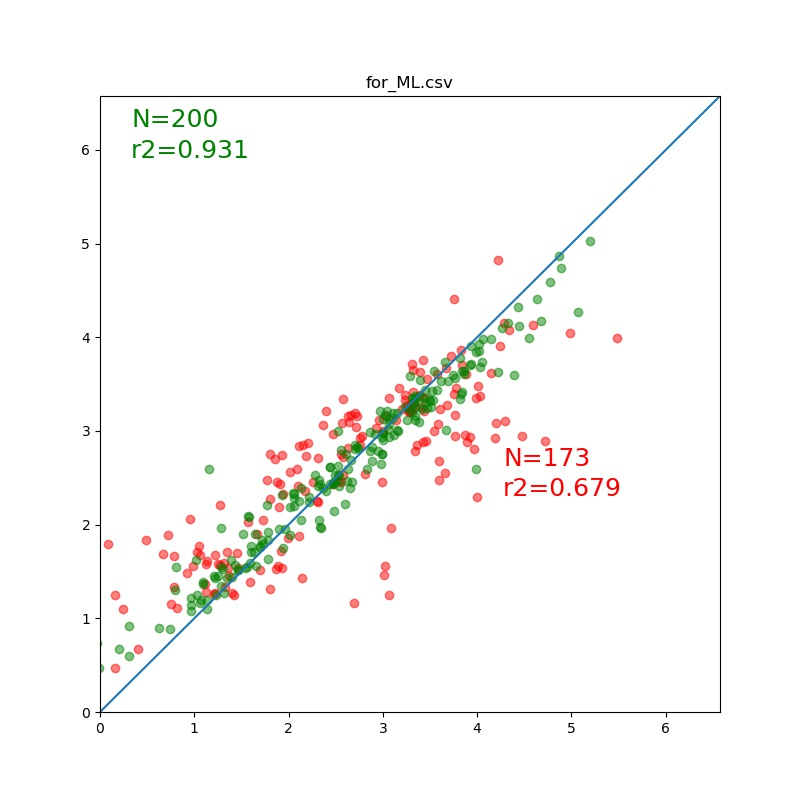
\includegraphics[width=\linewidth]{Results/2019-04-11/target=Average_Voltage.jpg}
        \caption{}
    \end{subfigure}
   % ~ 
    \begin{subfigure}{0.3\textwidth}
        \centering
        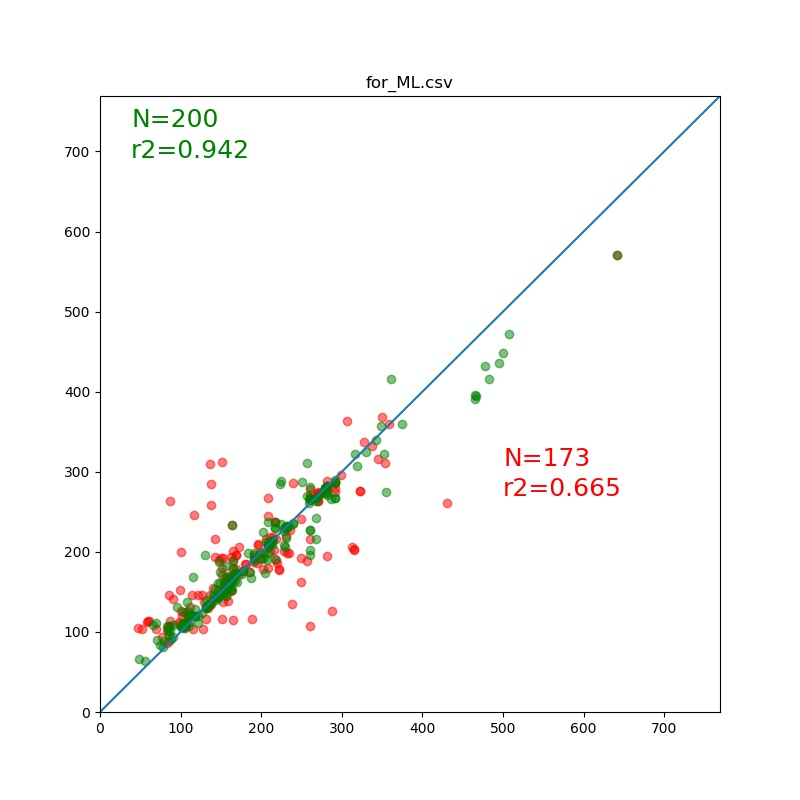
\includegraphics[width=\linewidth]{Results/2019-04-11/target=Capacity_Grav.jpg}
        \caption{}
    \end{subfigure}
       % ~ 
    \begin{subfigure}{0.3\textwidth}
        \centering
        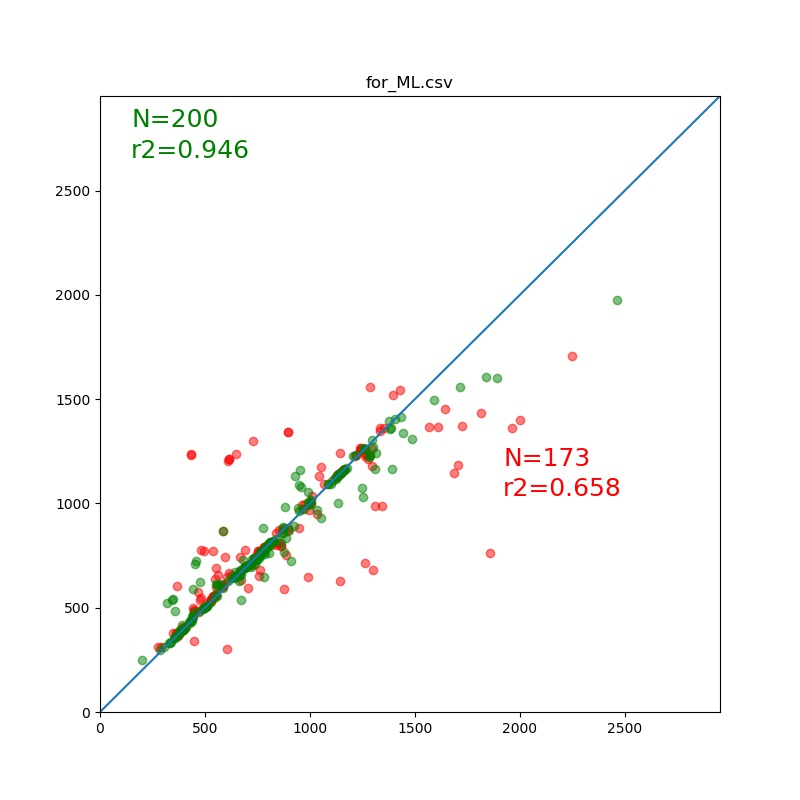
\includegraphics[width=\linewidth]{Results/2019-04-11/target=Capacity_Vol.jpg}
        \caption{}
    \end{subfigure}
       % ~ 
    \begin{subfigure}{0.3\textwidth}
        \centering
        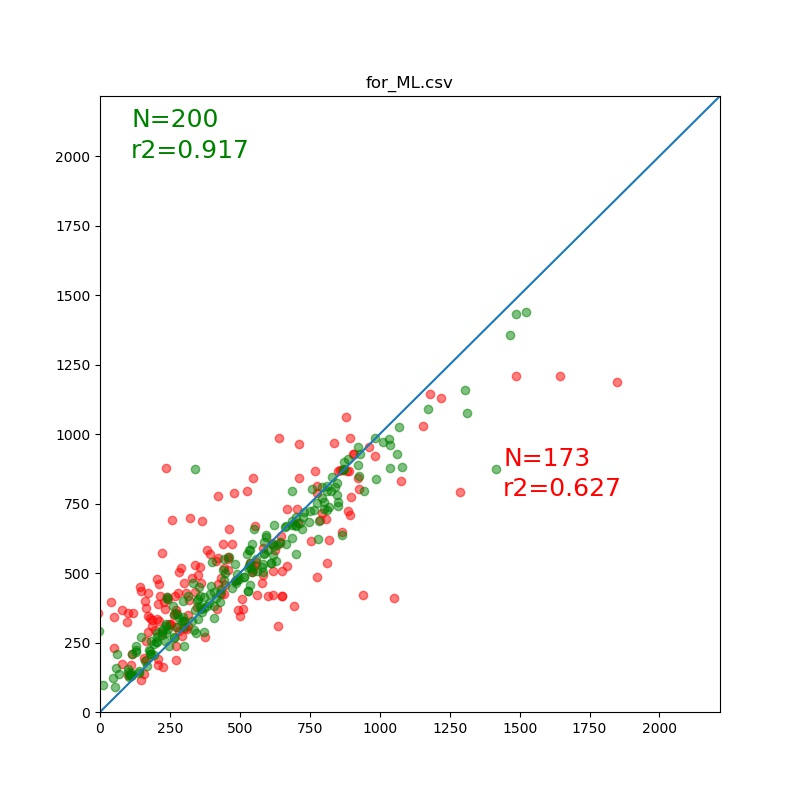
\includegraphics[width=\linewidth]{Results/2019-04-11/target=Specific_E_Wh_kg.jpg}
        \caption{}
    \end{subfigure}
       % ~ 
    \begin{subfigure}{0.3\textwidth}
        \centering
        \includegraphics[width=\linewidth]{Results/2019-04-11/target=E_Density_Wh_l.jpg}
            \caption{}
    \end{subfigure}
       % ~ 
    \begin{subfigure}{0.3\textwidth}
        \centering
        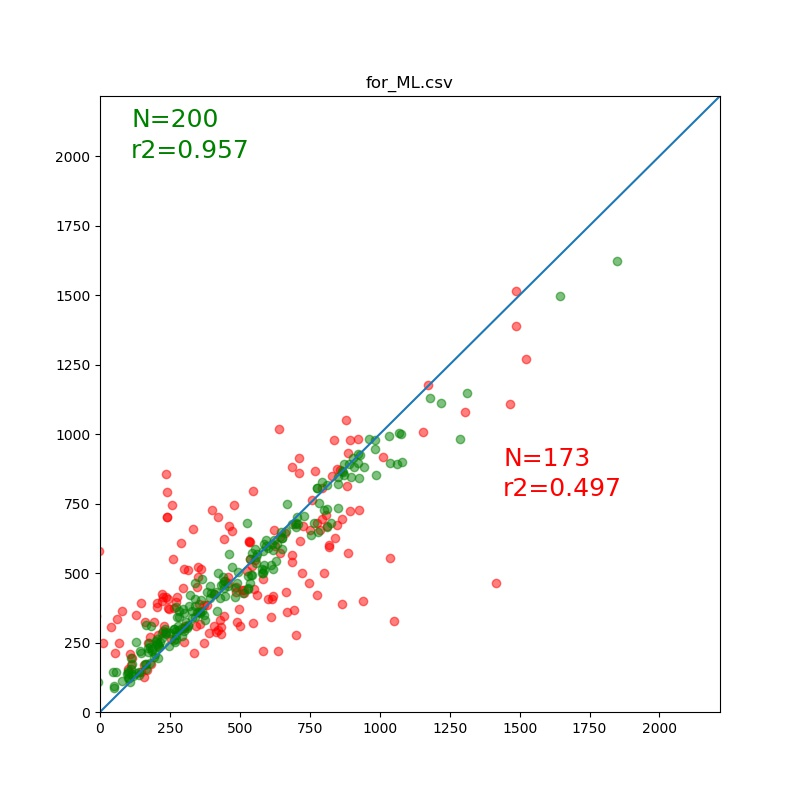
\includegraphics[width=\linewidth]{Results/2019-04-11/target=Stability_Discharge.jpg}
            \caption{}
    \end{subfigure}
\caption[R2 plot]{R2 plot for different runs}
    \label{fig:numberdensity_a-f}

\end{figure}

\subsection{Energy descriptions}

\begin{figure}
    \centering
    \includegraphics[width=\linewidth]{Results/plots/mean_crossvalidation_plot.png}
\caption[Cross validation and prediction uncertainty plot]{The Cross validation and the predictions uncertainty plottet for different runs with different predictors and the specific energy as the target for all runs. No removal of outliers have been implemented. l = number density, hgv = helvol, geomvol of void fraction, AV = average voltage, CGV = gravimetric and volumetric capacity, ED = energy density}
\label{fig:mean_cv}
\end{figure}
\myworries{}
\end{comment}


%Parameters.
%Volume number density
%Try to tell a STORY.


%Presentation between 30-45 minuttes. 

%Problem?
%method
%solution? 

% Test with density fraction:


% Test; weight of different parameters.

















\pagebreak
\part{Summary}
\section{Summary and future work}
\subsection{Batteries}
\subsection{future work}
\subsubsection{improving method}




\pagebreak
\printbibliography

%\section{Appendix}\label{sec:appendix}
%This is the Appendix!






%\begin{align*}
%&n \qquad &2^n - (-1)^n\\
%&n+1 \qquad &2^{n+1} - (-1)^{n+1} \\
%& &= 2(2^{n}) - (-1)^{n+1}\\
%& &= 2(2^{n} + (-1)^n  + (-1)^{n+1}) - (-1)^{n+1}\\
%& &= 2(2^{n} + (-1)^n  - (-1)^{n}) - (-1)^{n+1}\\
%& &= 2(2^{n}- (-1)^{n}) + 2(-1)^n  + (-1)^{n}\\
%& &= 2(2^{n}- (-1)^{n}) + 3(-1)^n \\
%\end{align*}



% \begin{figure}[H]
%     \centering
%     \begin{subfigure}{0.5\textwidth}
%         \centering
%         \includegraphics[width=\linewidth]{result/bilder/Tc/e-Tc}
%         \caption{}
%     \end{subfigure}%
%     ~ 
%     \begin{subfigure}{0.5\textwidth}
%         \centering
%         \includegraphics[width=\linewidth]{result/bilder/Tc/m-Tc}
%         \caption{}
%     \end{subfigure}
%     \caption{a) Shows how E behaves around $T_C$ b) Shows how |M| develops near $T_C$.}
%     \label{fig:tc-E-M}
% \end{figure}






% \begin{center}
% \label{tab:states-2x2-summary}
% \captionof{table}{The table shows a summary from table \ref{tab:states-2x2}. }
% \begin{tabularx}{\textwidth}{c X c X c X c}
%     \hline 
%     \hline 
%         Number of $\color{red}{\uparrow}$ && Multiplicity && Energy && Magnetic moment \\ 
%     \hline
%         4   &&      1      &&      -8J     &&       4       \\  
%         3   &&      4      &&      0J      &&       2       \\
%         2   &&      2      &&      8J      &&       0       \\
%         2   &&      4      &&      0J      &&       0       \\
%         1   &&      4      &&      0J      &&       -2      \\
%         0   &&      1      &&      -8J     &&       -4      \\
%     \hline
% \end{tabularx}
% \end{center}




%\begin{tabular}{|c|c|c|c|c|c|c|}
%	\hline 
%	n & General & Specific & LU & fastest & slowest & $\frac{slowest}{fastest}$\\ 
%	\hline
%	10 & 6.5e-05 & 5e-06 & 4e-05 & Specific & General & 13.0\\ 
%	\hline 
%	100 & 7.5e-05 & 8e-06 & 0.0023 & Specific & LU & 287.5\\ 
%	\hline 
%	1000 & 0.00014 & 4e-05 & 0.26 & Specific & LU & 6500\\ 
%	\hline
%	10000 & 0.0007 & 0.0005 & 142.5 & Specific & LU & 285000 \\ 
%	\hline
%\end{tabular}

%\begin{figure}[H]
%		\centering
%		\includegraphics[width=0.7\linewidth]{ab.png}
%		\caption{Atomene er gule kuler, de elementære vektorene er blå og a vektorene er grønne.}
%		\label{fig:ab}
%\end{figure}















\end{document}